\chapter{Results}
\label{chapter:results}
In this chapter we will implement all the models described before: constant volatility, Dupire's local volatility, Heston's stochastic volatility and both static and dynamic SABR models.

With the exception of Dupire's local volatility, will perform the calibration described in \autoref{section:Model Calibration} for all models: we will minimize the cost function in eq. \eqref{cost} with the weight function shown in eq. \eqref{weight}. The model values for the implied volatilities, $\sigma_{imp,\mathrm{mdl}}$, will be obtained through the closed form solutions for each of the models. We will apply the CMA-ES optimization algorithm to find the optimal solution.

To validate the models' closed-form solutions, after finding the optimal parameters we will input them into a Monte Carlo pricer (adapted to each model), and calculate the simulated option price with each model's calibrated parameters. This price will then be converted into an implied volatility (using eq.\eqref{impvolform}) in order for the simulation to be comparable to the data and the closed form solutions. To better grasp the behavior of the simulations we will repeat them a large number of times, $N_{\mathrm{reps}}$, averaging the results to produce a function - henceforth named \emph{simulated function} -  and extracting from them the 95\% confidence intervals of the simulations - these confidence intervals are obtained by sorting the simulated implied volatilities for each strike and extracting both the 95\% highest and the 5\% lowest.


We will fit all our functions to a dataset of implied volatilities for European options with different maturities and strike prices. This data was kindly provided by \emph{BNP Paribas} and is shown in \autoref{chapter:mktdata}.


For the case of Dupire's local volatility, because it is nonparametric, no calibration is required. Instead we must perform an interpolation in order to find the implied volatility surface from the data mentioned before and, with it, find the local volatility function. From this, we can easily obtain the prices of European options from the Monte Carlo pricer described in subsections \ref{subsection:Simulating stock prices} and \ref{subsection:Pricing options from simulations}. These prices (and their implied volatilities) can then be compared to their true market values. As for the stochastic volatility models above, we will also run the Monte Carlo pricer a large number of times, $N_{\mathrm{reps}}$, to produce the simulated function and its 95\% confidence intervals.


In order for the models to be comparable, we need to make sure that the same global parameters are used in all the adjustments and simulations, namely the initial stock price, $S_0$, the risk-free interest rate, $r$, the time step size (used in the Monte Carlo simulations), $\Delta t$, the number of pricer repetitions (to be averaged, producing the expected simulated function and the confidence intervals), $N_{\mathrm{reps}}$, and the number of paths simulated, $N_{\mathrm{paths}}$. Their values are shown in \autoref{tab:defaultparam}.
\begin{table}[H]
    \centering
        \renewcommand{\arraystretch}{0.8}
\begin{tabular}{@{}lcccr@{}}
\toprule
$S_0$($\EUR$) & $r$($\SI{}{\per\year}$) & $\Delta t$(days) & $N_{\mathrm{paths}}$ & $N_{\mathrm{reps}}$ \\ \midrule
1 & 0 & 0.5 & 100 000 & 100\\
\bottomrule
\end{tabular}
  \caption[Parameters used throughout all simulations.]{Parameters used throughout all simulations.}
  \label{tab:defaultparam}
\end{table}

The Monte Carlo pricers of each model will then be modified to price Barrier options instead of the European options used in the calibration. These results will be compared with one another, though no validation is possible due to a lack of data.



\section{Constant Volatility Model}
To find how well our models perform, we need some reference against which to compare them. One clear possibility is to assume a constant volatility throughout the options' duration, since this is the simplest possible case.

The equation that generates each stock price path is therefore given by
\begin{equation}
dS(t)=rS(t)dt+\sigma S(t)dW(t).
\end{equation}

Because we are fitting the volatility function - which, in this case, is a constant value - to a set of volatility data - which is not constant - these adjustments are expected to badly represent the data. Any other minimally decent model is expected to outperform this constant volatility benchmark.

With this constant volatility model, we can choose to fit the datasets with different maturities independently of one another or together in a single coupled dataset. In other words, we can do several fits, one for each maturity, or a single one, for all maturities together. The former will be useful when benchmarking the Static SABR model, since for that model the adjustments will also be performed independently (Static SABR performs badly for multiple maturities). The latter will be more appropriate when studying the remaining models - Dupire, Heston and Dynamic SABR - since these fit the whole implied volatility surface (i.e. multiple maturities together). Thus, both versions will be implemented and briefly studied.


\newpage
\subsection{Independent Fits}
We begin by presenting the results of fitting a constant volatility function to the sets of data with different maturities \emph{independently}.


In \autoref{fig:ConstVol} we show the plots of each fit along with the provided market data. We also present the simulated functions and the simulations' confidence intervals.
\begin{figure}[H]
  \begin{subfigmatrix}{2}
    \subfigure[$T=21$ days]{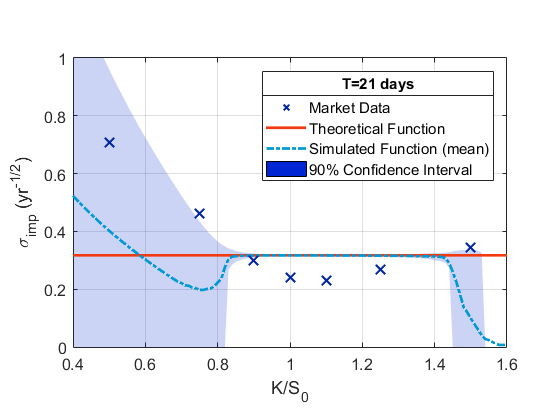
\includegraphics[width=0.49\linewidth,trim={0.25cm 0.45cm 1.1cm 1.4cm},clip]{ConstVol1.png}}
    \subfigure[$T=42$ days]{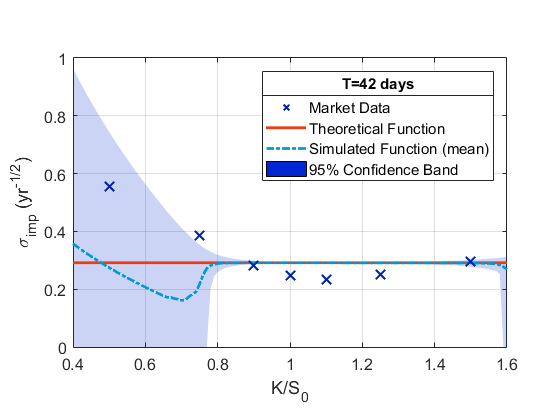
\includegraphics[width=0.49\linewidth,trim={0.25cm 0.45cm 1.1cm 1.4cm},clip]{ConstVol2.png}}
    \subfigure[$T=63$ days]{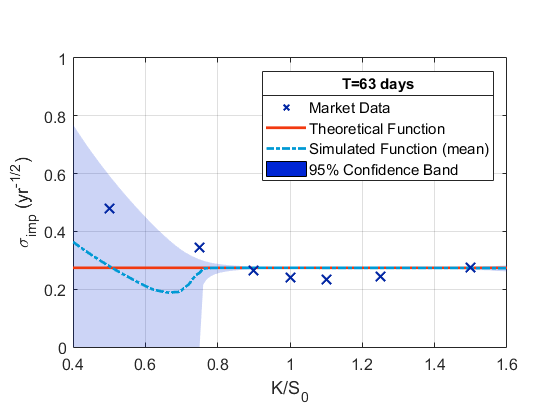
\includegraphics[width=0.49\linewidth,trim={0.25cm 0.45cm 1.1cm 1.4cm},clip]{ConstVol3.png}}
    \subfigure[$T=126$ days]{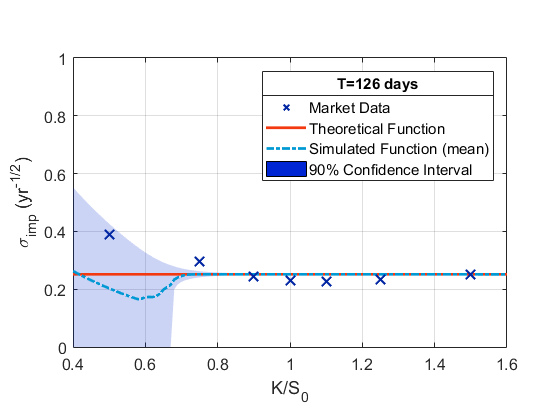
\includegraphics[width=0.49\linewidth,trim={0.25cm 0.45cm 1.1cm 1.4cm},clip]{ConstVol4.png}}
  \end{subfigmatrix}
  \caption[Implied volatility functions fitted independently to the implied volatility data for different maturities under constant volatility model, plotted with their respective Monte Carlo simulated functions along with their confidence intervals.]{Implied volatility functions (red lines) fitted \emph{independently} to the implied volatility data (crosses) for different maturities under constant volatility model, plotted with their respective Monte Carlo simulated functions (light-blue dot-dashed lines) along with their 95\% confidence intervals (blue region).}
  \label{fig:ConstVol}
\end{figure}

The fitted parameter, which, in this case, is only the constant implied volatility, is presented in \autoref{tab:ConstVolPar} for each of the maturities, along with the cost function's value (eq.\eqref{cost}) under this (fitted) model.

\begin{table}[H]
    \centering
        \renewcommand{\arraystretch}{0.8}
\begin{tabular}{@{}lcr@{}}
\toprule
$T$ (days) & $\sigma_{imp,\mathrm{mdl}}$ ($\SI{}{\year\tothe{-1/2}}$) & Cost \\ \midrule
21 & 0.3174 & 0.0635 \\
42 & 0.2918 & 0.0282 \\
63 & 0.2742 & 0.0164 \\
126& 0.2518 & 0.0069 \\
\bottomrule
\end{tabular}
  \caption[Fitted parameters for each maturity (fitted independently) under constant volatility model.]{Fitted parameters for each maturity (fitted independently) under constant volatility model.}
  \label{tab:ConstVolPar}
\end{table}


\begin{table}[H]
\centering
\renewcommand{\arraystretch}{0.8}
\begin{tabular}{@{}ccccSccS@{}}
\toprule
$T$(days) & $K$($\EUR$) & $\sigma_{i,\mathrm{mkt}}$($\SI{}{\year\tothe{-0.5}}$) &  $\sigma_{i,\mathrm{mdl}}$($\SI{}{\year\tothe{-0.5}}$) & \multicolumn{1}{c}{$\mathrm{Error}_{\sigma}(\%)$} & $C_{\mathrm{mkt}}$($\EUR$)&$C_{\mathrm{mdl}}$($\EUR$)& \multicolumn{1}{c}{$\mathrm{Error}_{C}(\%)$}\\ \midrule
\multirow{7}{*}{21} & 0.50 & 0.7082 & \multirow{7}{*}{0.3174} & 55.2 & 0.50001 & 0.50000 & 0.003 \\
&0.75 & 0.4632 &  & 31.5 & 0.25065 & 0.25002 & 0.3 \\
&0.90 & 0.2989 &  & 6.2 & 0.10439 & 0.10540 & 1.0 \\
&1.00 & 0.2425 &  & 30.9 & 0.02792 & 0.03654 & 30.9 \\
&1.10 & 0.2314 &  & 37.1 & 2.42$\times10^{-3}$ & 7.41$\times10^{-3}$ & 205.9 \\
&1.25 & 0.2699 &  & 17.6 & 5.34$\times10^{-5}$ & 25.01$\times10^{-5}$ & 367.9 \\
&1.50 & 0.3433 &  & 7.5 & 5.75$\times10^{-7}$ & 1.12$\times10^{-7}$ & 80.5 \\\midrule
\multirow{7}{*}{42}&0.50 & 0.5556 & \multirow{7}{*}{0.2918} & 47.5 & 0.50005 & 0.50000 & 0.01 \\
&0.75 & 0.3876 &  & 24.7 & 0.25186 & 0.25027 & 0.6 \\
&0.90 & 0.2824 &  & 3.3 & 0.11069 & 0.11166 & 0.9 \\
&1.00 & 0.2461 &  & 18.6 & 0.04006 & 0.04749 & 18.5 \\
&1.10 & 0.2354 &  & 23.9 & 8.52$\times10^{-3}$ & 15.00$\times10^{-3}$ & 75.9 \\
&1.25 & 0.2525 &  & 15.6 & 6.21$\times10^{-4}$ & 15.75$\times10^{-4}$ & 153.8 \\
&1.50 & 0.2968 &  & 1.7 & 1.58$\times10^{-5}$ & 1.24$\times10^{-5}$ & 21.4 \\\midrule
\multirow{7}{*}{63}&0.50 & 0.4789 &\multirow{7}{*}{0.2742}  & 42.7 & 0.50009 & 0.50000 & 0.02 \\
&0.75 & 0.3452 &  & 20.6 & 0.25296 & 0.25077 & 0.9 \\
&0.90 & 0.2658 &  & 3.2 & 0.11533 & 0.11650 & 1.0 \\
&1.00 & 0.2401 &  & 14.2 & 0.04787 & 0.05465 & 14.2 \\
&1.10 & 0.2330 &  & 17.7 & 0.01421 & 0.02069 & 45.5 \\
&1.25 & 0.2438 &  & 12.5 & 1.80$\times10^{-3}$ & 3.33$\times10^{-3}$ & 85.1 \\
&1.50 & 0.2749 &  & 0.3 & 7.66$\times10^{-5}$ & 7.44$\times10^{-5}$ & 2.9 \\\midrule
\multirow{7}{*}{126}&0.50 & 0.3878 &  \multirow{7}{*}{0.2518}& 35.1 & 0.50035 & 0.50000 & 0.07 \\
&0.75 & 0.2954 &  & 14.7 & 0.25694 & 0.25344 & 1.4 \\
&0.90 & 0.2444 &  & 3.1 & 0.12716 & 0.12882 & 1.3 \\
&1.00 & 0.2295 &  & 9.7 & 0.06467 & 0.07094 & 9.7 \\
&1.10 & 0.2269 &  & 11.0 & 0.02862 & 0.03488 & 21.9 \\
&1.25 & 0.2340 &  & 7.6 & 7.57$\times10^{-3}$ & 9.98$\times10^{-3}$ & 31.8 \\
&1.50 & 0.2521 &  & 0.1 & 8.58$\times10^{-4}$ & 8.51$\times10^{-4}$ & 0.8 \\
\bottomrule
\end{tabular}
  \caption[Comparison between fitted results (fitted independently) and original data under constant volatility model.]{Comparison between fitted functions (fitted independently) and original data under constant volatility model.}
  \label{tab:CV}
\end{table}

By observing the fit results in \autoref{tab:ConstVolPar} we see that the cost function decreases with the maturity. This is indeed what is expected, since the implied volatility surface becomes flatter as maturity increases, as can be seen from the market data (and also as we can see in \autoref{fig:DupImpV}), making the constant volatility function a better approximation in such cases, and decreasing the cost function's value.


One other property that we can observe is that the constant implied volatility also decreases with maturity. The reason behind this is the simple fact that earlier maturities contain higher implied volatilities, which pull the constant volatility function upwards.


We now focus on the simulated results in \autoref{fig:ConstVol}.

First, we can see that the theoretical functions (full red lines) clearly don't represent the market data. This is indeed what is expected. After all, if a constant volatility model was enough to price options, the more complex models would not be needed.

Secondly, by comparing the theoretical and simulated functions, we must note that the simulation performs extremely well for strikes near $S_0$. Notice that the simulated function (dot-dashed blue line) perfectly follows the constant volatility theoretical result (full red line) in this region, with the confidence intervals collapsed into the simulated function indicating that all simulations produced the same result. This suggests that the simulation is working as expected.

Thirdly, we notice that on the earliest maturity (i.e. 21 days), for strikes much larger than $S_0$ (e.g. $K=1.5S_0$), the simulated implied volatilities go to zero, even though they should remain constant. The reason behind this has already been discussed in \autoref{subsection:Pricing options from simulations} and relates to the very, very small number of paths that reach such high strikes and end up contributing to the option price (which is then converted to an implied volatility). For the case of strike $K=1.5S_0$, and maturity $T=21$ days, the number of paths that reach the strike is indeed approximately 0.25 out of 100000 - sometimes a single path is able to breach this strike, but usually none do. This problem is not observed for the remaining maturities for the simple reason that, because they are given more time to evolve, more paths are able to reach these high strikes.
To solve solve this problem we could significantly increase the number of simulations, so that the number of paths that are able to reach these high strikes is enough to produce a valid. The problem with this solution is the very significant increase in the computation time required, which makes it impractical.
If we lowered the number of simulated paths from 100000 paths to any other number, the problem described before would become even more aggravated, and the later maturities would also display the problem observed in the earliest maturity.

Finally we must discuss the large confidence intervals for strikes lower than $S_0$, occurring over all maturities. To explain this we require the information presented in \autoref{fig:ImpVolPrice}, relating the implied volatility with the option's market price. We saw that the implied volatility was extremely sensitive to option prices very close to their lower bounds, $S_0-Ke^{-rT}$. If we now look, for example, at the market price of the option with strike $K=\SI{0.5}{\EUR}$ and maturity $T=21$ days, which is $C=\SI{0.500013}{\EUR}$, and we compare it with its lower bound, $S_0-Ke^{-rT}=\SI{0.5}{\EUR}$, we can clearly see that they are extremely close, with a difference of only $0.0026\%$. We can then conclude that, in this case, we are in the extremely high sensitivity region of the implied volatility functions shown in \autoref{fig:ImpVolPrice}.
The Monte Carlo pricer behaves very well for the lower strikes since a very large number of paths contribute to the option price (the opposite of what we described before for high strikes). Despite this, because there will always be some noise associated with the simulations, the generated price is sure to present some very slight variation when executed multiple times, which is enough to cause some of the simulated implied volatilities to go to approximately zero (or to increase), which explains the large confidence intervals. For options with strikes near $S_0$ and above the market option price is much farther from its lower bound, so that we are above the high sensitivity region. Indeed, the lower bound of options with strikes equal to or above $S_0$ is 0 (assuming interest rate $r=0$).

These two last problems are not inherent to the constant volatility model. Indeed they will be observed, to some extent, in all the models we will study next.




\newpage

\subsection{Dependent Fits}
We now present the results obtained from the adjustment of a constant volatility function to all the implied volatility data, regardless of maturity.

In \autoref{fig:ConstVol2} are shown the theoretical and simulated functions as well as the provided market data.
\begin{figure}[H]
  \begin{subfigmatrix}{2}
    \subfigure[$T=21$ days]{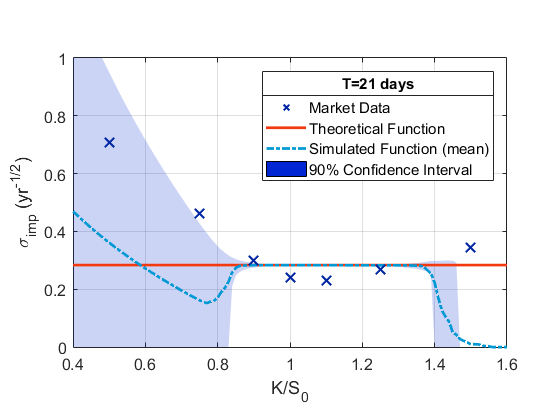
\includegraphics[width=0.49\linewidth,trim={0.25cm 0.45cm 1.1cm 1.4cm},clip]{ConstVol12.png}}
    \subfigure[$T=42$ days]{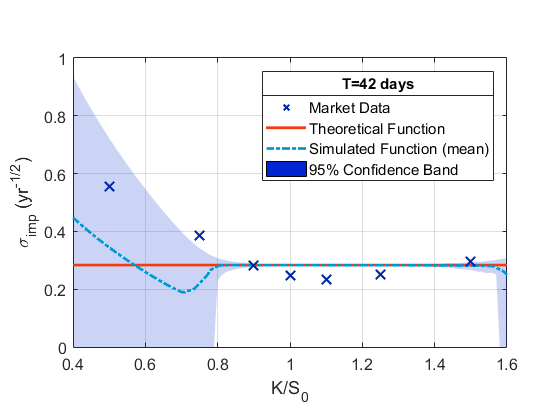
\includegraphics[width=0.49\linewidth,trim={0.25cm 0.45cm 1.1cm 1.4cm},clip]{ConstVol22.png}}
    \subfigure[$T=63$ days]{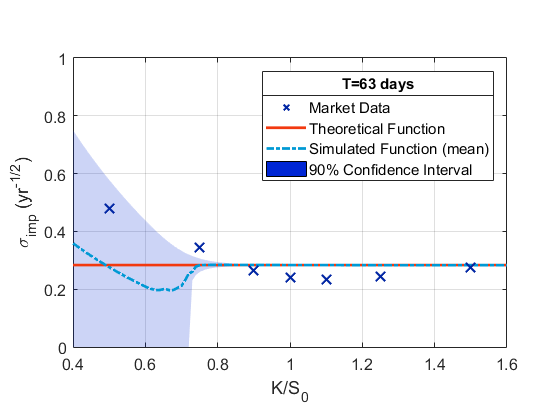
\includegraphics[width=0.49\linewidth,trim={0.25cm 0.45cm 1.1cm 1.4cm},clip]{ConstVol32.png}}
    \subfigure[$T=126$ days]{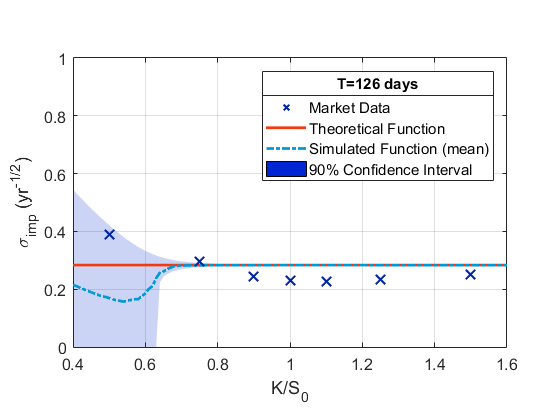
\includegraphics[width=0.49\linewidth,trim={0.25cm 0.45cm 1.1cm 1.4cm},clip]{ConstVol42.png}}
  \end{subfigmatrix}
  \caption[Implied volatility functions fitted simultaneously to the implied volatility data for different maturities under constant volatility model, plotted with their respective Monte Carlo simulated functions along with their confidence intervals.]{Implied volatility functions (red lines) fitted \emph{simultaneously} to the implied volatility data (crosses) for different maturities under constant volatility model, plotted with their respective Monte Carlo simulated functions (light-blue dot-dashed lines) along with their 95\% confidence intervals (blue region).}
  \label{fig:ConstVol2}
\end{figure}

The fitted implied volatility is represented in \autoref{tab:ConstVolPar2} as well as the cost function's value.
\begin{table}[H]
    \centering
        \renewcommand{\arraystretch}{0.8}
\begin{tabular}{@{}lr@{}}
\toprule
 $\sigma_{imp,\mathrm{mdl}}$ ($\SI{}{\year\tothe{-1/2}}$) & Cost \\ \midrule
0.2838 & 0.1248 \\
\bottomrule
\end{tabular}
  \caption[Fitted parameters for all maturities (fitted simultaneously) under constant volatility model.]{Fitted parameters for all maturities (fitted simultaneously) under constant volatility model.}
  \label{tab:ConstVolPar2}
\end{table}


\begin{table}[H]
\centering
\renewcommand{\arraystretch}{0.8}
\begin{tabular}{@{}ccccSccS@{}}
\toprule
$T$(days) & $K$($\EUR$) & $\sigma_{i,\mathrm{mkt}}$($\SI{}{\year\tothe{-0.5}}$) &  $\sigma_{i,\mathrm{mdl}}$($\SI{}{\year\tothe{-0.5}}$) & \multicolumn{1}{c}{$\mathrm{Error}_{\sigma}(\%)$} & $C_{\mathrm{mkt}}$($\EUR$)&$C_{\mathrm{mdl}}$($\EUR$)& \multicolumn{1}{c}{$\mathrm{Error}_{C}(\%)$}\\ \midrule
\multirow{7}{*}{21} & 0.50 & 0.7082 & \multirow{7}{*}{0.2838} & 59.9 & 0.50001 & 0.50000 & 0.003 \\
 & 0.75 & 0.4632 &  & 38.7 & 0.25065 & 0.25000 & 0.3 \\
 & 0.90 & 0.2989 &  & 5.0 & 0.10439 & 0.10364 & 0.7 \\
 & 1.00 & 0.2425 &  & 17.0 & 0.02792 & 0.03267 & 17.0 \\
 & 1.10 & 0.2314 &  & 22.6 & 2.42$\times10^{-3}$ & 5.19$\times10^{-3}$ & 114.4 \\
 & 1.25 & 0.2699 &  & 5.1 & 5.34$\times10^{-5}$ & 8.98$\times10^{-5}$ & 67.9 \\
 & 1.50 & 0.3433 &  & 17.3 & 5.75$\times10^{-7}$ & 0.07$\times10^{-7}$ & 98.8 \\\midrule
\multirow{7}{*}{42} & 0.50 & 0.5556 & \multirow{7}{*}{0.2838} & 48.9 & 0.50005 & 0.50000 & 0.01 \\
 & 0.75 & 0.3876 &  & 26.8 & 0.25186 & 0.25021 & 0.7 \\
 & 0.90 & 0.2824 &  & 0.5 & 0.11069 & 0.11084 & 0.1 \\
 & 1.00 & 0.2461 &  & 15.3 & 0.04006 & 0.04620 & 15.3 \\
 & 1.10 & 0.2354 &  & 20.6 & 8.52$\times10^{-3}$ & 14.02$\times10^{-3}$ & 64.5 \\
 & 1.25 & 0.2525 &  & 12.4 & 6.21$\times10^{-4}$ & 13.36$\times10^{-4}$ & 115.3 \\
 & 1.50 & 0.2968 &  & 4.4 & 1.58$\times10^{-5}$ & 0.83$\times10^{-5}$ & 47.6 \\\midrule
\multirow{7}{*}{63} & 0.50 & 0.4789 & \multirow{7}{*}{0.2838} & 40.7 & 0.50009 & 0.50000 & 0.02 \\
 & 0.75 & 0.3452 && 17.8 & 0.25296 & 0.25097 & 0.8 \\
 & 0.90 & 0.2658 && 6.8 & 0.11533 & 0.11786 & 2.2 \\
 & 1.00 & 0.2401 && 18.2 & 0.04787 & 0.05656 & 18.2 \\
 & 1.10 & 0.2330 && 21.8 & 0.01421 & 0.02227 & 56.7 \\
 & 1.25 & 0.2438 && 16.4 & 1.80$\times10^{-3}$ & 3.93$\times10^{-3}$ & 118.2 \\
 & 1.50 & 0.2749 && 3.2 & 7.66$\times10^{-5}$ & 10.87$\times10^{-5}$ & 42.0 \\\midrule
\multirow{7}{*}{126} & 0.50 & 0.3878 & \multirow{7}{*}{0.2838} & 26.8 & 0.50035 & 0.50001 & 0.1 \\
 & 0.75 & 0.2954 && 3.9 & 0.25694 & 0.25589 & 0.4 \\
 & 0.90 & 0.2444 && 16.1 & 0.12716 & 0.13611 & 7.0 \\
 & 1.00 & 0.2295 && 23.7 & 0.06467 & 0.07992 & 23.6 \\
 & 1.10 & 0.2269 && 25.1 & 0.02862 & 0.04317 & 50.8 \\
 & 1.25 & 0.2340 && 21.3 & 7.57$\times10^{-3}$ & 14.99$\times10^{-3}$ & 98.0 \\
 & 1.50 & 0.2521 && 12.6 & 8.58$\times10^{-4}$ & 19.67$\times10^{-4}$ & 129.3 \\
\bottomrule
\end{tabular}
  \caption[Comparison between fitted results (fitted simultaneously) and original data under constant volatility model.]{Comparison between fitted functions (fitted simultaneously) and original data under constant volatility model.}
  \label{tab:CV2}
\end{table}


First, when we compare the implied volatility fitted to all the maturities with the results of the independent fits (in \autoref{tab:ConstVolPar}) we see that the former is actually the average of the latter. \hl{why?}

If we now compare the cost function values, we see that the cost of the dependent fit ($0.1248$), is actually larger than the sum of cost of the independent fits ($0.0635+0.0282+0.0164+0.0069=0.1150$). This is indeed expected: when fitting all maturities at once, the optimizer will find the implied volatility that minimizes the cost for all maturities, which will not be the one that minimizes the cost of each single maturity, so that the sum of the errors is higher.

As for the plots in \autoref{fig:ConstVol2} they look very similar to those in \autoref{fig:ConstVol}, so not much more can be added regarding their analysis.





\newpage
\section{Dupire Model}
The stochastic differential equation for the stock price paths under the local volatility model was hypothesized to be given by
\begin{equation}\label{dupmodds}
dS(t)=rS(t)dt+\sigma(S(t),t)S(t)dW(t),
\end{equation}
\noindent where $\sigma(S(t),t)$ can be obtained through Dupire's model, defined in \autoref{subsection:Dupire}, which is given by
\begin{equation}
\sigma(S(t),t)=\sqrt{\frac{\displaystyle\sigma_{imp}^2+2t\sigma_{imp}\pdv{\sigma_{imp}}{T}+2r(S(t))t\sigma_{imp}\pdv{\sigma_{imp}}{K}}{\displaystyle\left(1+(S(t))d_1\sqrt{t}\pdv{\sigma_{imp}}{K}\right)^2+(S(t))^2t\sigma_{imp}\left(\pdv{^2\sigma_{imp}}{K^2}-d_1\left(\pdv{\sigma_{imp}}{K}\right)^2\sqrt{t}\right)}},
\end{equation}
\noindent where $d_1$ is defined as
\begin{equation}
d_1=\frac{\log(S_0/S(t))+\left(r+\frac{1}{2}\sigma_{imp}^2\right)t}{\sigma_{imp}\sqrt{t}}.
\end{equation}

As we mentioned in \autoref{section:Surface Interpolation (Dupire)}, we must produce the implied volatility surface from the market data using an interpolation algorithm. Applying the Delaunay triangulation defined earlier, we obtain the implied volatility surface shown in \autoref{fig:DupImpV}, along with its contour plot.
From this surface we can easily extract (numerically) the gradients required for the local volatility formula.



\begin{figure}[H]
  \begin{subfigmatrix}{2}
    \subfigure[$\sigma_{imp}$ surface]{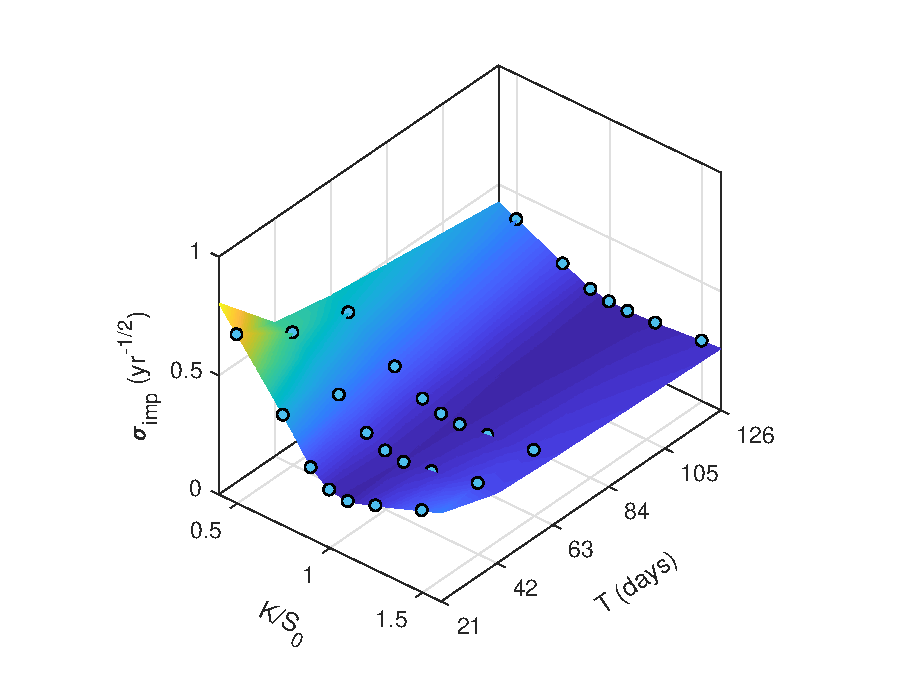
\includegraphics[width=0.49\linewidth,trim={1.7cm 0.45cm 2.cm 0.85cm},clip]{ImpliedV.eps}}
    \subfigure[$\sigma_{imp}$ contour plot]{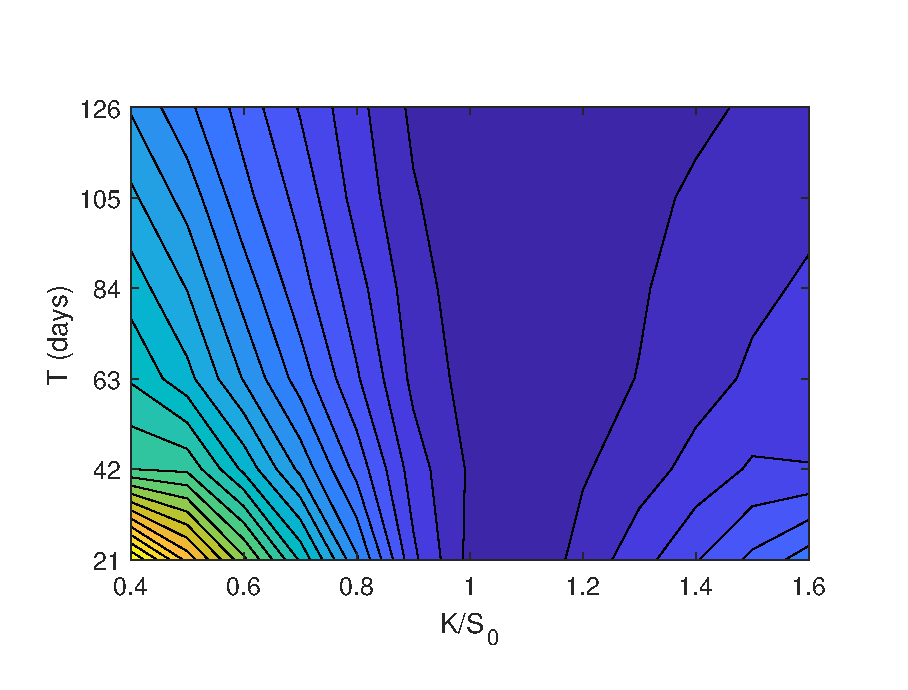
\includegraphics[width=0.49\linewidth,trim={0.2cm 0.5cm 1.25cm 1.55cm},clip]{ImpliedVC.eps}}
  \end{subfigmatrix}
    \caption[Implied volatility surface and corresponding contour plot of the function interpolated linearly between the original data points using Delaunay triangulation.]{Implied volatility surface (left) and corresponding contour plot (right) of the function interpolated linearly between the original data points (blue circles) using Delaunay triangulation.}\label{fig:DupImpV}
\end{figure}   


Observing this interpolated surface we see that its curvature decreases with maturity - the volatility smile becomes less prominent for later maturities.


We now should now be able to generate the \emph{local} volatility surface. To do this, we simply evaluate the interpolated implied volatility surface, as well as all the required gradients, at multiple points $K_j$, $T_i$ to produce the local volatility $\sigma(K_j,T_i)$. The points should be uniformly spaced in a grid - with $K_min$ and $K_max$ being the smallest and largest strike $K_j$ in the grid, with intervals $\Delta K$ between the strikes, and with $T_min$ and $T_max$ the smallest and largest maturity $T_i$, with intervals $\Delta T$. These parameters are shown in \autoref{tab:DupR}.
Interpolating again between these points we are able to generate the local volatility surface, shown in \autoref{fig:DupLocVol}. We now simply need to make a variable change $\sigma(K,T)\implies \sigma(S,t)$ to be able to input this value into eq.\eqref{dupmodds}.


\begin{table}[H]
    \centering
        \renewcommand{\arraystretch}{0.8}
\begin{tabular}{@{}cccccc@{}}
\toprule
$T_{min}$(days) & $T_{max}$(days) & $\Delta T$(days) & $K_{min}$($\EUR$) & $K_{max}$($\EUR$) & \multicolumn{1}{c}{$\Delta K$($\EUR$)}\\ \midrule
21 & 126 & 10.5 & 0.4 & 1.6 & \multicolumn{1}{c}{0.05} \\ \bottomrule
\end{tabular}
  \caption[Parameters used in the interpolation section of Dupire's model.]{Parameters used in the interpolation section of Dupire's model.}
  \label{tab:DupR}
\end{table}


\begin{figure}[H]
  \begin{subfigmatrix}{2}
    \subfigure[$\sigma_{loc}$ surface]{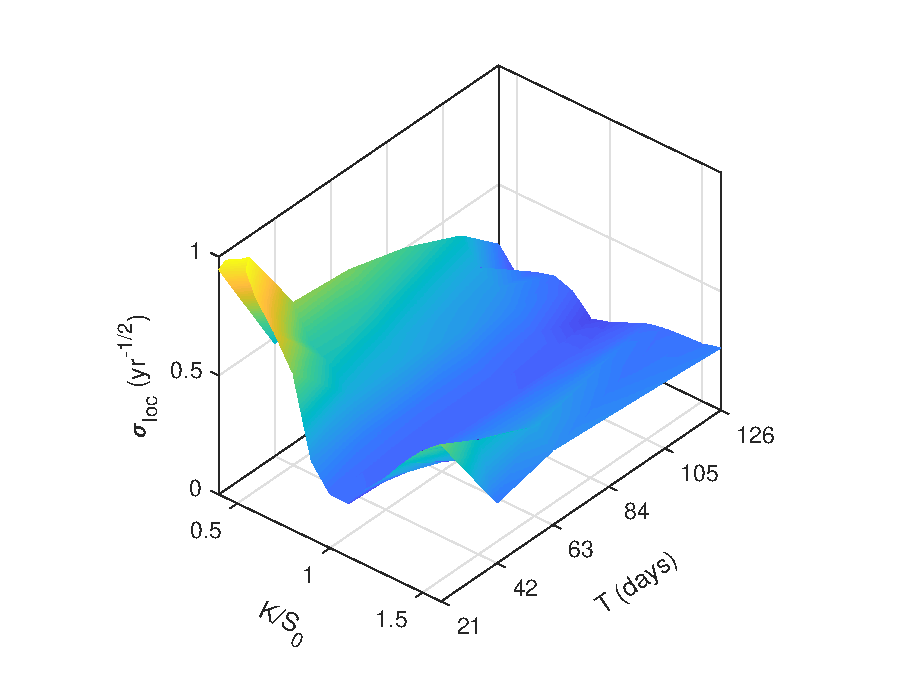
\includegraphics[width=0.49\linewidth,trim={1.7cm 0.45cm 2.cm 0.85cm},clip]{LocalV.eps}}
    \subfigure[$\sigma_{loc}$ contour plot]{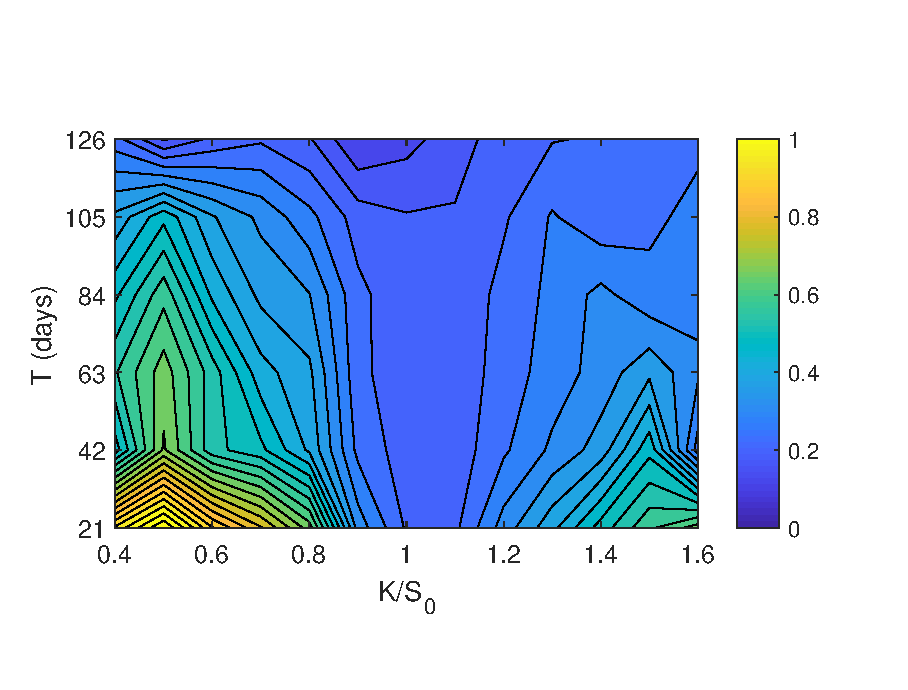
\includegraphics[width=0.49\linewidth,trim={0.2cm 0.5cm 1.25cm 1.55cm},clip]{LocalVC.eps}}
  \end{subfigmatrix}
    \caption[Local volatility surface and corresponding contour plot of the function obtained with Dupire's formula from the interpolated implied volatility surface.]{Local volatility surface (left) and corresponding contour plot (right) of the function obtained with Dupire's formula (eq.\eqref{dupire2}) from the interpolated implied volatility surface in \autoref{fig:DupImpV}.}\label{fig:DupLocVol}
\end{figure}   

Having obtained the local volatility surface, simulating the stock price paths is quite easy. We just need evaluate the surface at the point $(S_i,t_j)$ when we are at the time step $t_j$ of the simulation with a stock price path at $S_i$. To price options, we now simply need to apply the Monte Carlo pricing algorithm. The results of such simulations is shown in \autoref{fig:Dup}, along with the confidence intervals and the original market data. To prevent volatilities from becoming too high we implemented a maximum cutoff value of $\sigma_{max}$=$\SI{1.5}{\year\tothe{-1/2}}$, limiting the volatilities obtained from the surface.

\vspace{\fill}
\newpage

\begin{figure}[H]
  \begin{subfigmatrix}{2}
    \subfigure[$T=21$ days]{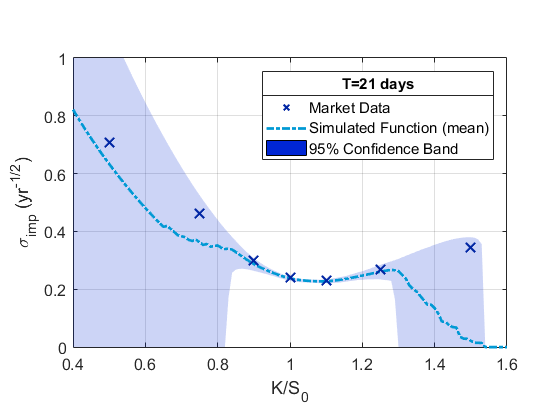
\includegraphics[width=0.49\linewidth,trim={0.25cm 0.45cm 1.1cm 1.4cm},clip]{Dup1.png}}
    \subfigure[$T=42$ days]{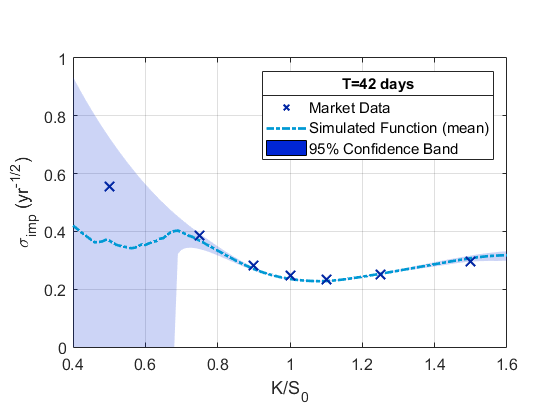
\includegraphics[width=0.49\linewidth,trim={0.25cm 0.45cm 1.1cm 1.4cm},clip]{Dup2.png}}
    \subfigure[$T=63$ days]{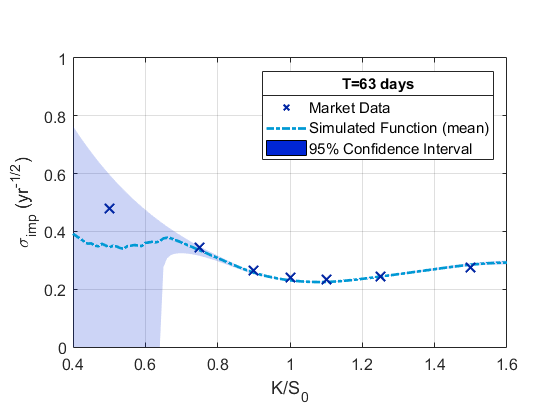
\includegraphics[width=0.49\linewidth,trim={0.25cm 0.45cm 1.1cm 1.4cm},clip]{Dup3.png}}
    \subfigure[$T=126$ days]{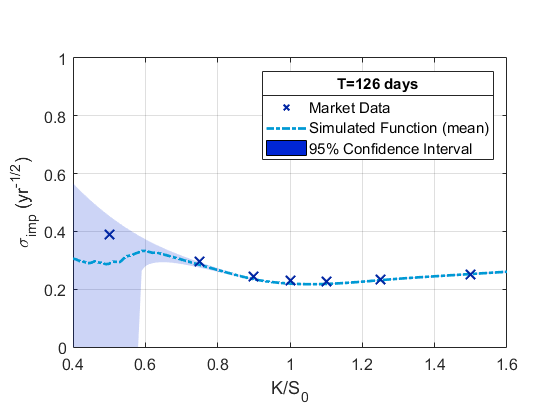
\includegraphics[width=0.49\linewidth,trim={0.25cm 0.45cm 1.1cm 1.4cm},clip]{Dup4.png}}
  \end{subfigmatrix}
  \caption[Implied volatility functions simulated with Monte Carlo under Dupire's local volatility model with their corresponding 95\% confidence interval, plotted against the original market data.]{Implied volatility functions (light-blue dot-dashed) simulated with Monte Carlo under Dupire's local volatility model with their corresponding 95\% confidence interval, plotted against the original market data (crosses).}
  \label{fig:Dup}
\end{figure}


As before, we now see the very large confidence intervals for very low strikes. The cause of this behavior was identified on the constant volatility model (with independent fits). Also here we can see the low implied volatilities for high strikes in the earliest maturities. This has also already been discussed.

The great improvement of Dupire's model over the constant volatility model is the presence of the implied volatility smiles in the simulated implied volatilities. Furthermore, these smiles follow the market data almost perfectly for strikes near $S_0$.
We can therefore conclude that the model greatly outperforms the constant volatility model presented earlier.

The plots shown in \autoref{fig:Dup} can be thought of as slices of a simulated implied volatility surface. Ideally, this surface would look exactly like the one shown in \autoref{fig:DupImpV}. However, because we are now simulating the prices, there should exist some variation. Furthermore, in the regions where the pricer performs badly (i.e. large strikes for early maturities and low strikes), we expect there to be a very high amount of noise. This simulated surface is shown in \autoref{fig:DupS}, along with the simulated functions of the earlier plots.



\begin{figure}[H]
  \begin{subfigmatrix}{2}
    \subfigure[$\sigma_{imp}$ surface]{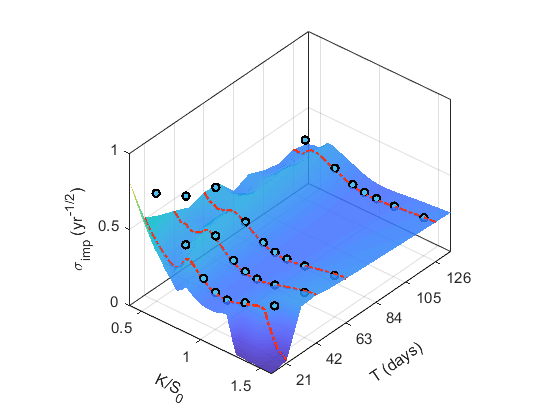
\includegraphics[width=0.49\linewidth,trim={1.7cm 0.45cm 1.9cm 0.85cm},clip]{DupS.png}}
    \subfigure[$\sigma_{imp}$ contour plot]{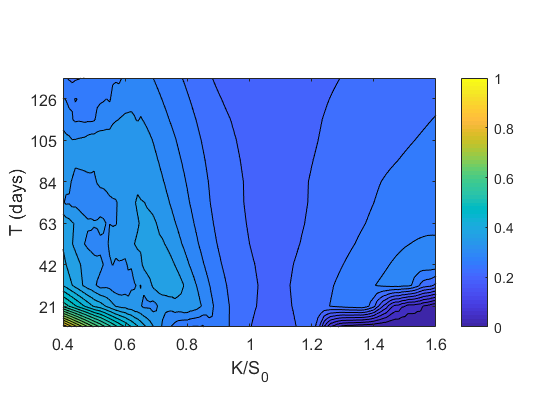
\includegraphics[width=0.49\linewidth,trim={0.2cm 0.5cm 1.25cm 1.55cm},clip]{DupSC.png}}
  \end{subfigmatrix}
    \caption[Implied volatility surface and corresponding contour plot simulated with Monte Carlo under Dupire's local volatility model plotted against the original market data and the generated functions shown in \autoref{fig:Dup}.]{Implied volatility surface (left) and corresponding contour plot (right) simulated with Monte Carlo under Dupire's local volatility model plotted against the original market data (blue circles) and the generated functions shown in \autoref{fig:Dup} (red dot-dashed lines).}\label{fig:DupS}
\end{figure}   


As expected, the amount of noise is quite overwhelming in the regions where the Monte Carlo pricer performs badly. For the regions where the strike approaches $S_0$, the behavior is quite different and the simulations closely follow the data, as expected.

\vspace{\fill}
\newpage

\begin{table}[H]
\centering
\renewcommand{\arraystretch}{0.8}
\begin{tabular}{@{}ccccSccS@{}}
\toprule
$T$(days) & $K$($\EUR$) & $\sigma_{i,\mathrm{mkt}}$($\SI{}{\year\tothe{-0.5}}$) &  $\sigma_{i,\mathrm{mdl}}$($\SI{}{\year\tothe{-0.5}}$) & \multicolumn{1}{c}{$\mathrm{Error}_{\sigma}(\%)$} & $C_{\mathrm{mkt}}$($\EUR$)&$C_{\mathrm{mdl}}$($\EUR$)& \multicolumn{1}{c}{$\mathrm{Error}_{C}(\%)$}\\ \midrule
\multirow{7}{*}{21} & 0.50 & 0.7082 & 0.2319 & 67.3 & 0.50001 & 0.50000 & 0.003 \\
 & 0.75 & 0.4632 & 0.3740 & 19.3 & 0.25065 & 0.25011 & 0.2 \\
 & 0.90 & 0.2989 & 0.2845 & 4.8 & 0.10439 & 0.10368 & 0.7 \\
 & 1.00 & 0.2425 & 0.2374 & 2.1 & 0.02792 & 0.02734 & 2.1 \\
 & 1.10 & 0.2314 & 0.2276 & 1.7 & 2.42$\times10^{-3}$ & 2.26$\times10^{-3}$ & 6.8 \\
 & 1.25 & 0.2699 & 0.2633 & 2.5 & 5.34$\times10^{-5}$ & 4.06$\times10^{-5}$ & 24.0 \\
 & 1.50 & 0.3433 & 0.1421 & 58.6 & 5.75$\times10^{-7}$ & 0 & 100.0 \\\midrule
\multirow{7}{*}{42} & 0.50 & 0.5556 & 0.3846 & 30.8 & 0.50005 & 0.50000 & 0.01 \\
 & 0.75 & 0.3876 & 0.3683 & 5.0 & 0.25186 & 0.25139 & 0.2 \\
 & 0.90 & 0.2824 & 0.2700 & 4.4 & 0.11069 & 0.10946 & 1.1 \\
 & 1.00 & 0.2461 & 0.2358 & 4.2 & 0.04006 & 0.03838 & 4.2 \\
 & 1.10 & 0.2354 & 0.2286 & 2.9 & 8.52$\times10^{-3}$ & 7.83$\times10^{-3}$ & 8.2 \\
 & 1.25 & 0.2525 & 0.2539 & 0.6 & 6.21$\times10^{-4}$ & 6.46$\times10^{-4}$ & 4.1 \\
 & 1.50 & 0.2968 & 0.3089 & 4.1 & 1.58$\times10^{-5}$ & 2.70$\times10^{-5}$ & 70.3 \\\midrule
\multirow{7}{*}{63} & 0.50 & 0.4789 & 0.3176 & 33.7 & 0.50009 & 0.50000 & 0.02 \\
 & 0.75 & 0.3452 & 0.3355 & 2.8 & 0.25296 & 0.25256 & 0.2 \\
 & 0.90 & 0.2658 & 0.2578 & 3.0 & 0.11533 & 0.11424 & 0.9 \\
 & 1.00 & 0.2401 & 0.2310 & 3.8 & 0.04787 & 0.04606 & 3.8 \\
 & 1.10 & 0.2330 & 0.2253 & 3.3 & 0.01421 & 0.01307 & 8.0 \\
 & 1.25 & 0.2438 & 0.2440 & 0.1 & 1.80$\times10^{-3}$ & 1.81$\times10^{-3}$ & 0.5 \\
 & 1.50 & 0.2749 & 0.2845 & 3.5 & 7.66$\times10^{-5}$ & 11.15$\times10^{-5}$ & 45.7 \\\midrule
\multirow{7}{*}{126} & 0.50 & 0.3878 & 0.3870 & 0.2 & 0.50035 & 0.50035 & 0.001 \\
 & 0.75 & 0.2954 & 0.2876 & 2.6 & 0.25694 & 0.25623 & 0.3 \\
 & 0.90 & 0.2444 & 0.2358 & 3.5 & 0.12716 & 0.12528 & 1.5 \\
 & 1.00 & 0.2295 & 0.2203 & 4.0 & 0.06467 & 0.06207 & 4.0 \\
 & 1.10 & 0.2269 & 0.2190 & 3.5 & 0.02862 & 0.02667 & 6.8 \\
 & 1.25 & 0.2340 & 0.2319 & 0.9 & 7.57$\times10^{-3}$ & 7.31$\times10^{-3}$ & 3.4 \\
 & 1.50 & 0.2521 & 0.2528 & 0.3 & 8.58$\times10^{-4}$ & 8.77$\times10^{-4}$ & 2.2 \\
 \bottomrule
\end{tabular}
  \caption[Comparison between the data obtained by generating $N_{paths}$ paths under Dupire's local volatility model using the Monte Carlo pricing method and the original data.]{Comparison between the data obtained by generating $N_{paths}$ paths under Dupire's local volatility model using the Monte Carlo pricing method and the original data.}
  \label{tab:Dup}
\end{table}










\newpage
\section{Static SABR Model}
As we saw before, the Static SABR model is defined as
\begin{equation}
dS(t)=rS(t)dt+e^{-r(T-t)(1-\beta)}\sigma(t)(S(t))^\beta dW_1(t),
\end{equation}
\begin{equation}
d\sigma(t)=\nu\sigma(t) dW_2(t),
\end{equation}
\noindent with $\alpha=\sigma(0)$ and with $W_1(t)$ and $W_2(t)$ having a constant correlation of $\rho$.

The closed form solution, shown in eq.\eqref{sabr}, enables us to obtain the theoretical implied volatilities of options priced under this model and will be used in the calibration process.

Before calibrating the model to the market data, we should study the influence of each parameter of this model on the shape of the implied volatility curve, in order to better interpret the results. This influence is represented in \autoref{fig:SSparam}, where we vary a single parameter at a time, keeping all the others constant, thus directly observing that parameter's influence.


We should note that the influence of the parameters is more complicated than we show here. On the one hand, their impact depends on the maturity. However, for this effect to become evident, we would have to repeat all the plots in \autoref{fig:SSparam} for several maturities, which would simply become too cumbersome and is out of the scope of this thesis.
On the other hand, the parameters have correlated effects on the curve shape. These influences would be quite difficult to represent. Furthermore, they are discussed in the original article by Hagan~\citep{Hagan}, and will, for these reasons, not be discussed here.
That being said, we can still have a general view of each parameter's impact on the curve.

\vspace{\fill}
\newpage

\begin{figure}[H]
  \begin{subfigmatrix}{2}
    \subfigure[Dependence on $\alpha$]{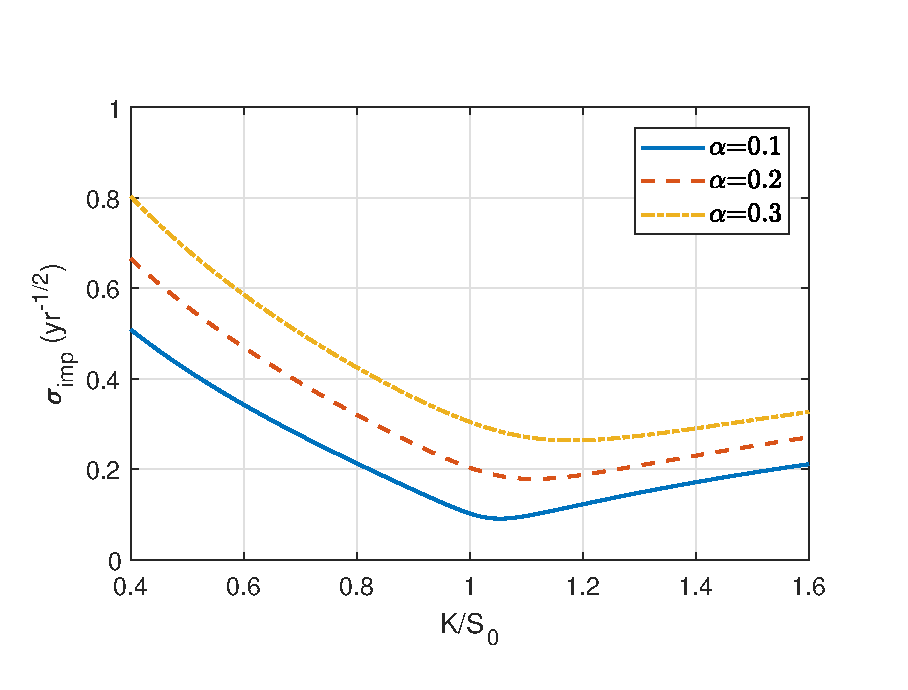
\includegraphics[width=0.49\linewidth,trim={0.25cm 0.45cm 1.1cm 1.4cm},clip]{SSalpha.eps}\label{SSa}}
    \subfigure[Dependence on $\beta$]{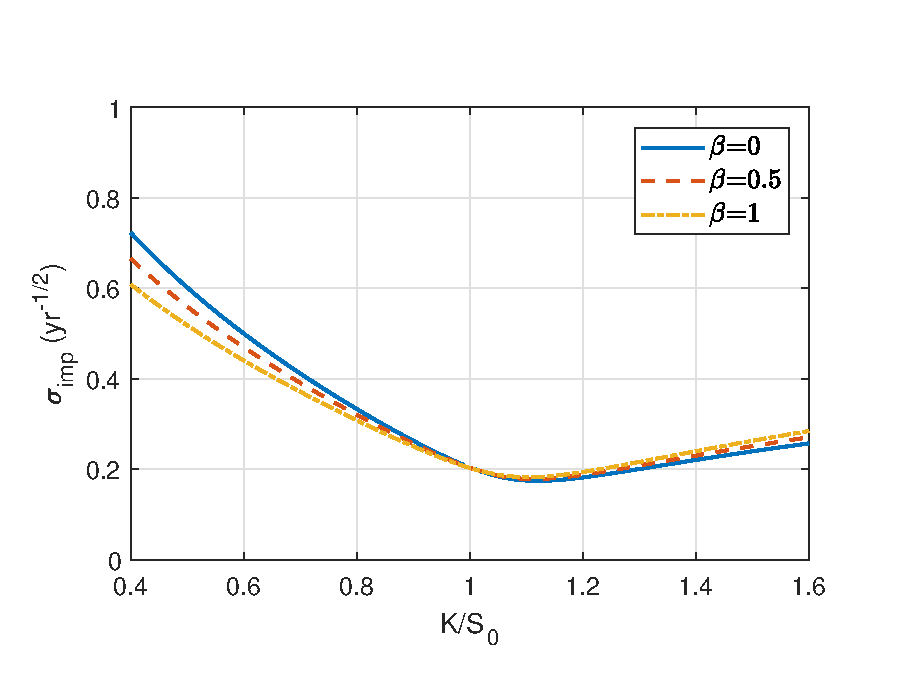
\includegraphics[width=0.49\linewidth,trim={0.25cm 0.45cm 1.1cm 1.4cm},clip]{SSbeta.eps}\label{SSb}}
    \subfigure[Dependence on $\rho$]{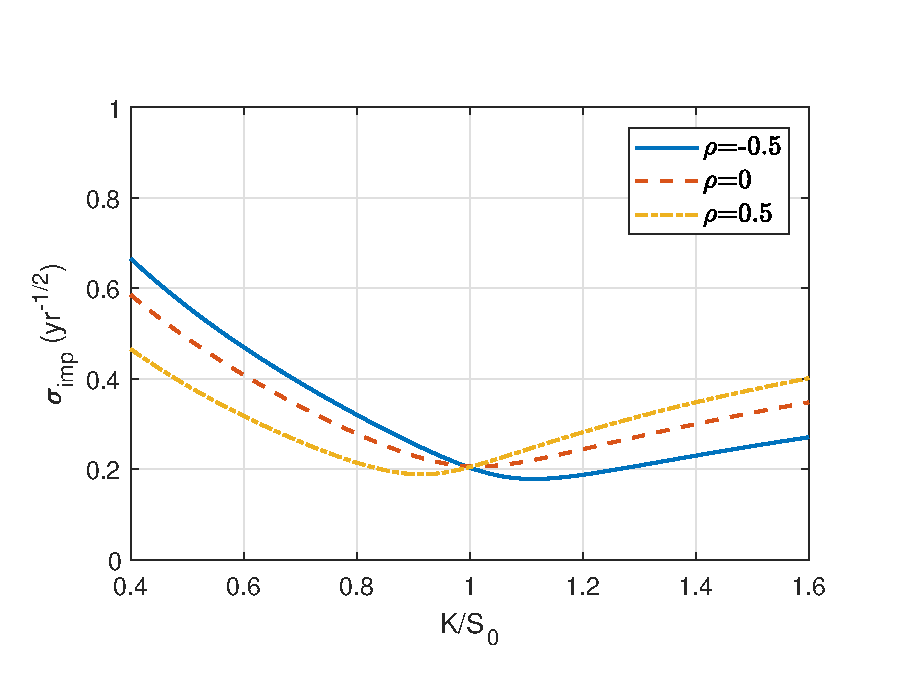
\includegraphics[width=0.49\linewidth,trim={0.25cm 0.45cm 1.1cm 1.4cm},clip]{SSrho.eps}\label{SSr}}
    \subfigure[Dependence on $\nu$]{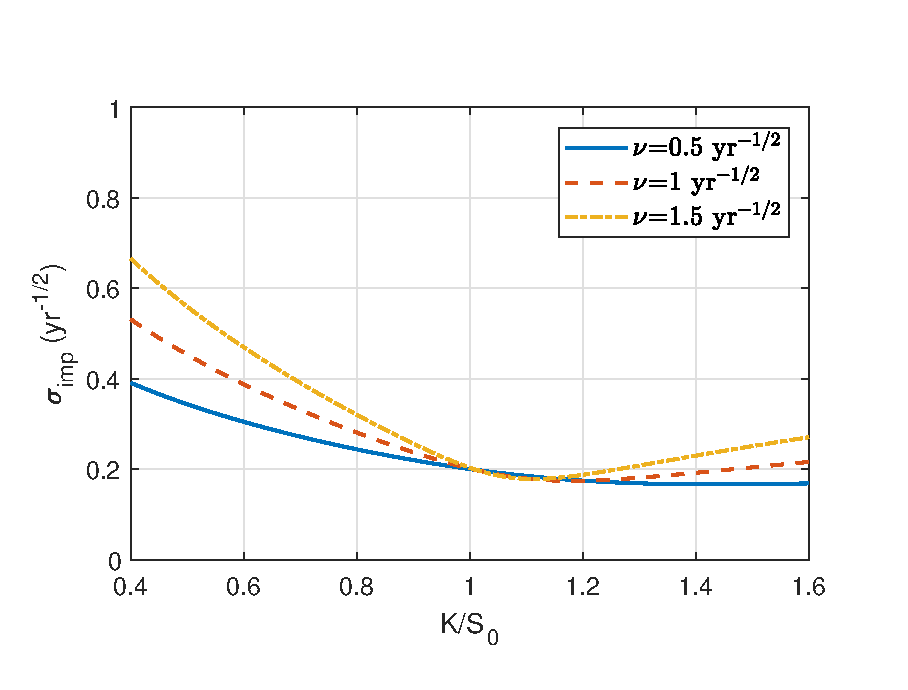
\includegraphics[width=0.49\linewidth,trim={0.25cm 0.45cm 1.1cm 1.4cm},clip]{SSnu.eps}\label{SSn}}
  \end{subfigmatrix}
  \caption[Dependence of the implied volatility curve on each of the Static SABR model parameters.]{Dependence of the implied volatility curve on each of the Static model SABR parameters. The default parameters used were $S_0=1\EUR$, $T=42$ days and $r=0$. Furthermore, on all plots, except when the dependence on a parameter is represented, the parameters used were $\alpha=0.2$, $\beta=1$, $\rho=-0.5$ and $\nu=1.5$.}
  \label{fig:SSparam}
\end{figure}

In Figure \autoref{SSa} we see that the parameter $\alpha$, which corresponds to the initial value of the volatility process, has quite an impact on the implied volatility curve. This parameter essentially controls the height of the curve. This is indeed expected, because the implied volatility and the stochastic (local) volatility are inherently related. Increasing $\alpha$ is expected to shift the volatility process to higher values, thus increasing the implied volatility.

The influence of the parameter $\beta$, which is an exponent in the stock price process, is represented in Figure \autoref{SSb}. The impact of this parameter seems to be almost negligible. Indeed, at a single point in time, the implied volatility curve barely changes, but this parameter becomes very important when time passes and the stock prices move (as they do when being simulated), because it controls how the curve shifts when such movements occur. If the stock price increases, the implied volatility curve at that time should shifts to the right. For $\beta=0$, the curve also shifts downwards, whereas for $\beta=1$ it doesn't. This behavior is studied in detail in the original article by Hagan~\citep{Hagan}.
Despite this, because in Static SABR we are only fitting data for a single maturity, this parameter should barely have any influence in the resulting implied volatility function, though it will become quite relevant in the Dynamic SABR model.

In Figure \autoref{SSr} is represented the effect of the parameter $\rho$, the correlation between the stock price and the volatility processes.
We can see that this parameter impacts the skewness of the implied volatility curve. Because this parameter relates the stock price and volatility, in the case of a negative $\rho$ when the prices increase (decrease), the volatilities decrease (increase), so that options with higher (lower) strikes have lower (higher) associated volatilities. This justifies why we have a lower implied volatility for higher strikes when the correlation is negative.

Finally, the impact of the parameter $\nu$, the volatility of the volatility process, is shown in Figure \autoref{SSn}. This parameter seems to control the curvature of the implied volatility curve. It should be clear that higher values of $\nu$ result in greater changes in the volatility process, enabling, at times, the volatility to become quite large. This allows the stock price process to evolve quite erratically, thus making it easier for stock prices to reach higher values, making high strike options more valuable. This effect pushes their implied volatility upwards. The inverse effect also holds and a low $\nu$ will force the stochastic volatility process to become quite limited, preventing the stock prices from changing too much, and restraining them from reaching high strikes, pulling the implied volatility curve downwards.


We now present the results of the calibration as well as the simulations in \autoref{fig:SS}.

\begin{figure}[H]
  \begin{subfigmatrix}{2}
    \subfigure[$T=21$ days]{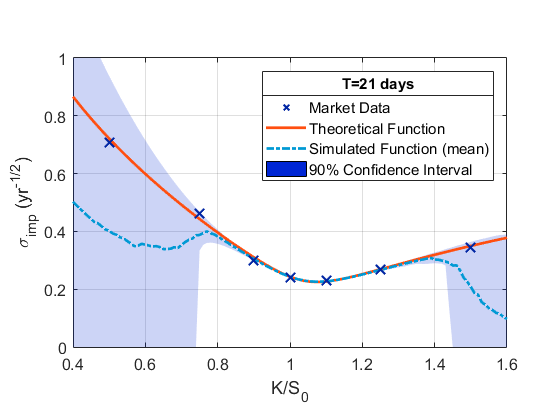
\includegraphics[width=0.49\linewidth,trim={0.25cm 0.45cm 1.1cm 1.4cm},clip]{SSABR1.png}}
    \subfigure[$T=42$ days]{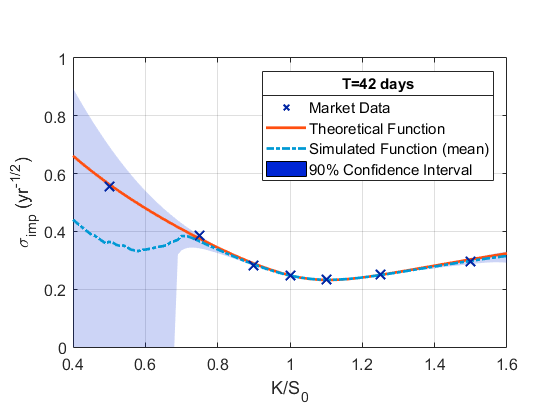
\includegraphics[width=0.49\linewidth,trim={0.25cm 0.45cm 1.1cm 1.4cm},clip]{SSABR2.png}}
    \subfigure[$T=63$ days]{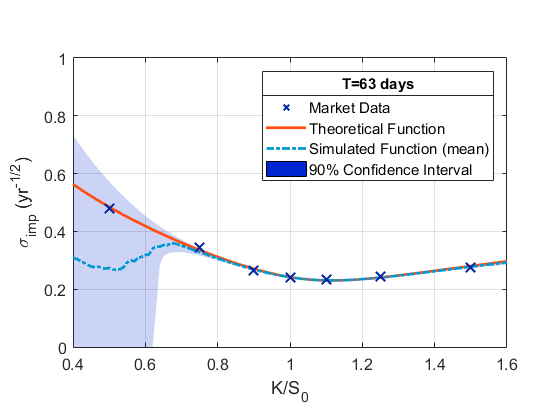
\includegraphics[width=0.49\linewidth,trim={0.25cm 0.45cm 1.1cm 1.4cm},clip]{SSABR3.png}}
    \subfigure[$T=126$ days]{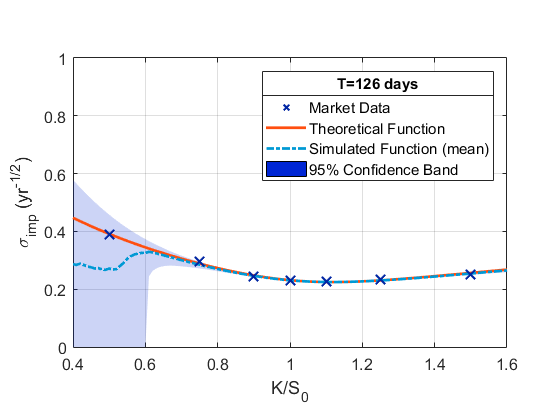
\includegraphics[width=0.49\linewidth,trim={0.25cm 0.45cm 1.1cm 1.4cm},clip]{SSABR4.png}}
  \end{subfigmatrix}
  \caption[Implied volatility functions fitted independently to the implied volatility data for different maturities under the static SABR model, plotted with their respective Monte Carlo simulated functions along with their 95\% confidence intervals.]{Implied volatility functions (red lines) fitted independently to the implied volatility data (crosses) for different maturities under the static SABR model, plotted with their respective Monte Carlo simulated functions (light-blue dot-dashed lines) along with their 95\% confidence intervals (blue region).}
  \label{fig:SS}
\end{figure}

As mentioned before, the Static SABR model is only expected to work for data on options with a single maturity. For this reason, the fits were done independently of one another.
The parameters obtained in the calibration for each of the maturities are shown in \autoref{tab:SSR}.

\begin{table}[H]
    \centering
        \renewcommand{\arraystretch}{0.8}
\begin{tabular}{@{}lccccr@{}}
\toprule
 $T$(days) & $\alpha$ ($\SI{}{\year\tothe{-1/2}}$) & $\beta$ & $\rho$ & $\nu$ & Cost \\ \midrule
21 & 0.2381 & 0.3766 & -0.3760 & 2.1022 & 0.000415 \\
42 & 0.2434 & 0.7362 & -0.3664 & 1.4451 & 0.000166\\
63 & 0.2375 & 0.7750 & -0.3119 & 1.1420 & 0.000102\\
126& 0.2267 & 0.8771 & -0.2383 & 0.8215 & 0.000055\\
\bottomrule
\end{tabular}
  \caption[Fitted parameters for each maturity (fitted independently) under static SABR model.]{Fitted parameters for each maturity (fitted independently) under static SABR model.}
  \label{tab:SSR}
\end{table}


We now analyze the results of this model. Observing the plots in \autoref{fig:SS} we see that the theoretical function, obtained by the closed form solution of the Static SABR model, fits the data extremely well through the whole range of strikes and for each of the maturities.

Though the model seems to fit almost perfectly to the data, the fits may not be very robust. The reason for this is that we have an extremely small amount of data points (7 for each maturity) for the comparatively large number of parameters used (4 parameters in total). This will cause our model to overfit the data.

As for the simulated function, we note that it very closely follows the theoretical curve in the regions around $S_0$, indicating that the Monte Carlo pricer implementation was done correctly. This feature doesn't hold at the high strike region in the first maturity and the low strike regions of all maturities for the same reasons described earlier.

Examining now the calibrated parameters in \autoref{tab:SSR} we first note that the parameter $\alpha$ doesn't seem to vary too much between maturities, which is expected, since it controls the height of the implied volatility curve, which doesn't seem to change too much in the plots.

The parameter $\beta$ appears to change wildly between maturities, though this is not surprising since, as we saw, this parameter doesn't significantly affect the shape of the implied volatility function.

As for the parameter $\rho$, we first note that it is always negative, which is expected from reality. It also seems to decrease with time \hl{why?}.

Finally, the parameter $\nu$ also seems to decrease with time. This is no surprise as the curvature of the implied volatility function is expected to decrease with time, with the function becoming increasingly horizontal.


If we now compare the cost function values of the Static SABR model in \autoref{tab:SSR} with the independently fitted results of the constant volatility assumption in \autoref{tab:ConstVolPar2} we clearly see that they improve very significantly. The cost decreases between 99.2 and 99.4\%, which is an extreme improvement. This is no surprise, since the constant volatility model was expected to perform very badly. These costs should be examined carefully, however, due to the overfitting mentioned earlier - for such a low amount of data relative to the great number of parameters we can find combinations of parameters that decrease the costs significantly, though they might not have any real interpretation.

\begin{table}[H]
\centering
\renewcommand{\arraystretch}{0.8}
\begin{tabular}{@{}ccccSccS@{}}
\toprule
$T$(days) & $K$($\EUR$) & $\sigma_{i,\mathrm{mkt}}$($\SI{}{\year\tothe{-0.5}}$) &  $\sigma_{i,\mathrm{mdl}}$($\SI{}{\year\tothe{-0.5}}$) & \multicolumn{1}{c}{$\mathrm{Error}_{\sigma}(\%)$} & $C_{\mathrm{mkt}}$($\EUR$)&$C_{\mathrm{mdl}}$($\EUR$)& \multicolumn{1}{c}{$\mathrm{Error}_{C}(\%)$}\\ \midrule
\multirow{7}{*}{21} & 0.50 & 0.7082 & 0.7209 & 1.8 & 0.50001 & 0.50002 & 0.001 \\
&0.75 & 0.4632 & 0.4428 & 4.4 & 0.25065 & 0.25047 & 0.1 \\
&0.90 & 0.2989 & 0.3105 & 3.9 & 0.10439 & 0.10501 & 0.6 \\
&1.00 & 0.2425 & 0.2435 & 0.4 & 0.02792 & 0.02804 & 0.4 \\
&1.10 & 0.2314 & 0.2269 & 2.0 & 2.42$\times10^{-3}$ & 2.23$\times10^{-3}$ & 8.0 \\
&1.25 & 0.2699 & 0.2692 & 0.3 & 5.34$\times10^{-5}$ & 5.18$\times10^{-5}$ & 3.0 \\
&1.50 & 0.3433 & 0.3500 & 1.9 & 5.75$\times10^{-7}$ & 8.32$\times10^{-7}$ & 44.7 \\\midrule
\multirow{7}{*}{42} &0.50 & 0.5556 & 0.5631 & 1.4 & 0.50005 & 0.50006 & 0.002 \\
&0.75 & 0.3876 & 0.3751 & 3.2 & 0.25186 & 0.25155 & 0.1 \\
&0.90 & 0.2824 & 0.2891 & 2.4 & 0.11069 & 0.11139 & 0.6 \\
&1.00 & 0.2461 & 0.2481 & 0.8 & 0.04006 & 0.04039 & 0.8 \\
&1.10 & 0.2354 & 0.2322 & 1.4 & 8.52$\times10^{-3}$ & 8.19$\times10^{-3}$ & 3.9 \\
&1.25 & 0.2525 & 0.2497 & 1.1 & 6.21$\times10^{-4}$ & 5.75$\times10^{-4}$ & 7.4 \\
&1.50 & 0.2968 & 0.3033 & 2.2 & 1.58$\times10^{-5}$ & 2.12$\times10^{-5}$ & 33.9 \\\midrule
\multirow{7}{*}{63} &0.50 & 0.4789 & 0.4845 & 1.2 & 0.50009 & 0.50011 & 0.002 \\
&0.75 & 0.3452 & 0.3357 & 2.8 & 0.25296 & 0.25256 & 0.2 \\
&0.90 & 0.2658 & 0.2710 & 2.0 & 0.11533 & 0.11605 & 0.6 \\
&1.00 & 0.2401 & 0.2421 & 0.8 & 0.04787 & 0.04826 & 0.8 \\
&1.10 & 0.2330 & 0.2305 & 1.1 & 0.01421 & 0.01384 & 2.6 \\
&1.25 & 0.2438 & 0.2409 & 1.2 & 1.80$\times10^{-3}$ & 1.68$\times10^{-3}$ & 6.7 \\
&1.50 & 0.2749 & 0.2804 & 2.0 & 7.66$\times10^{-5}$ & 9.56$\times10^{-5}$ & 24.8 \\\midrule
\multirow{7}{*}{126} &0.50 & 0.3878 & 0.3914 & 0.9 & 0.50035 & 0.50038 & 0.006 \\
&0.75 & 0.2954 & 0.2887 & 2.2 & 0.25694 & 0.25633 & 0.2 \\
&0.90 & 0.2444 & 0.2479 & 1.5 & 0.12716 & 0.12794 & 0.6 \\
&1.00 & 0.2295 & 0.2314 & 0.8 & 0.06467 & 0.06522 & 0.8 \\
&1.10 & 0.2269 & 0.2251 & 0.8 & 0.02862 & 0.02817 & 1.6 \\
&1.25 & 0.2340 & 0.2309 & 1.3 & 7.57$\times10^{-3}$ & 7.18$\times10^{-3}$ & 5.2 \\
&1.50 & 0.2521 & 0.2567 & 1.8 & 8.58$\times10^{-4}$ & 9.82$\times10^{-4}$ & 14.5 \\
 \bottomrule
\end{tabular}
  \caption[Comparison between fitted results and original data under static SABR model.]{Comparison between fitted results and original data under static SABR model.}
  \label{tab:SS}
\end{table}







\newpage
\section{Heston Model}
The Heston model is defined as
\begin{equation}
dS(t)=rS(t)dt+\sqrt{\nu(t)}S(t)dW_1(t),
\end{equation}
\begin{equation}
d\nu(t)=\kappa(\overline{\nu}-\nu(t))dt+\eta\sqrt{\nu(t)}dW_2(t),
\end{equation}
\noindent where $\nu_0=\nu(0)$ and with $W_1(t)$ and $W_2(t)$ having a constant correlation of $\rho$.

With the closed form solution of the Heston model, shown in eq.\eqref{CH}, we are able to find the theoretical prices of options priced under this model, which we can easily convert to implied volatilities. These last will be used in the calibration process.

As we did for the Static SABR model, we now study the influence of each parameter of the Heston model on the shape of the implied volatility curve, which is represented in \autoref{fig:Hparam}.

\begin{figure}[H]
  \begin{subfigmatrix}{2}
    \subfigure[Dependence on $\kappa$]{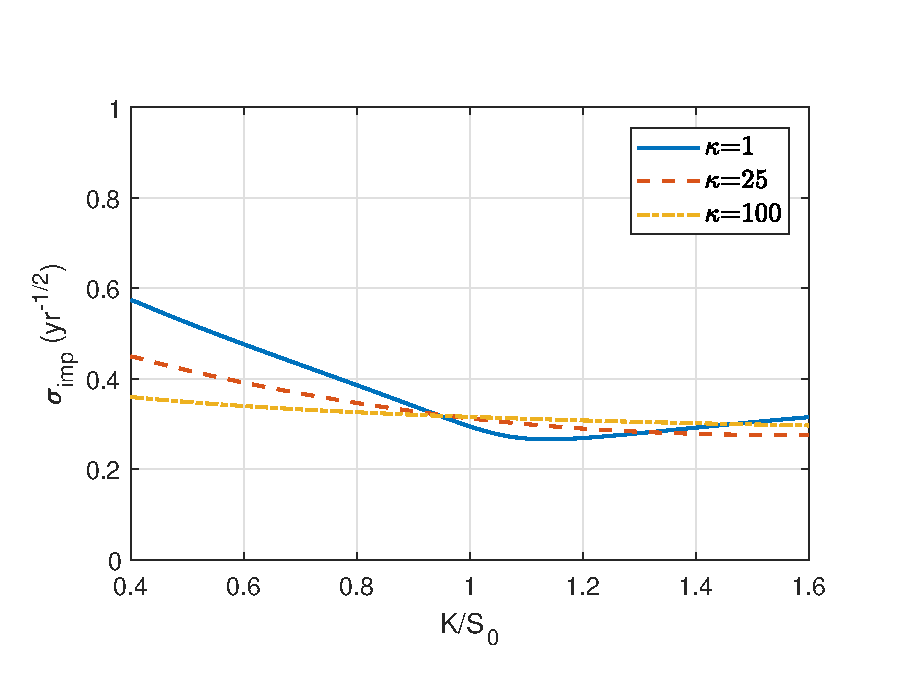
\includegraphics[width=0.49\linewidth,trim={0.25cm 0.45cm 1.1cm 1.4cm},clip]{Hkappa.eps}\label{Hk}}
    \subfigure[Dependence on $\overline{\nu}$]{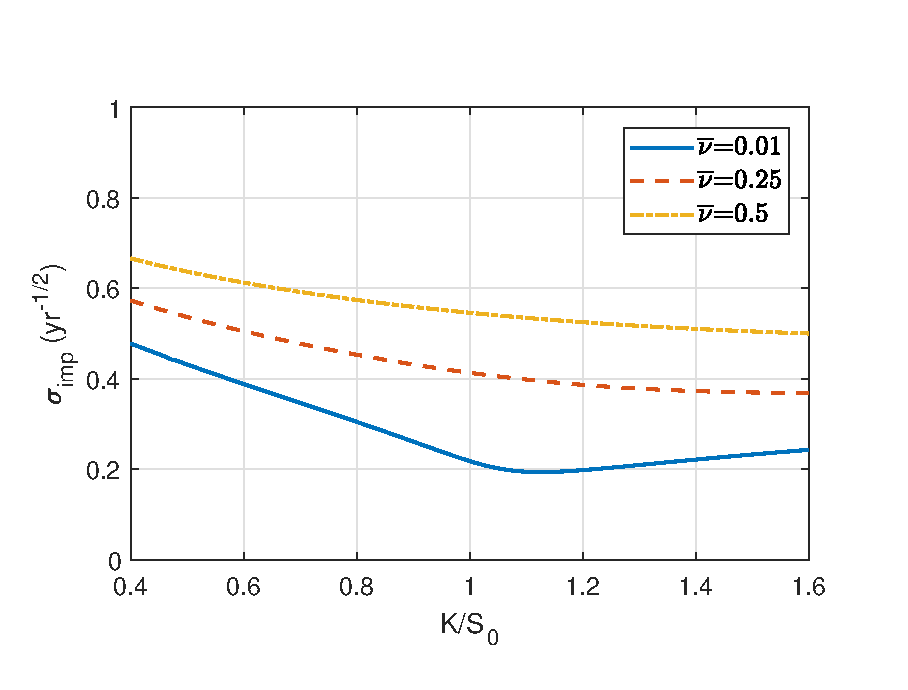
\includegraphics[width=0.49\linewidth,trim={0.25cm 0.45cm 1.1cm 1.4cm},clip]{Hnubar.eps}\label{Hnb}}
    \subfigure[Dependence on $\nu_0$]{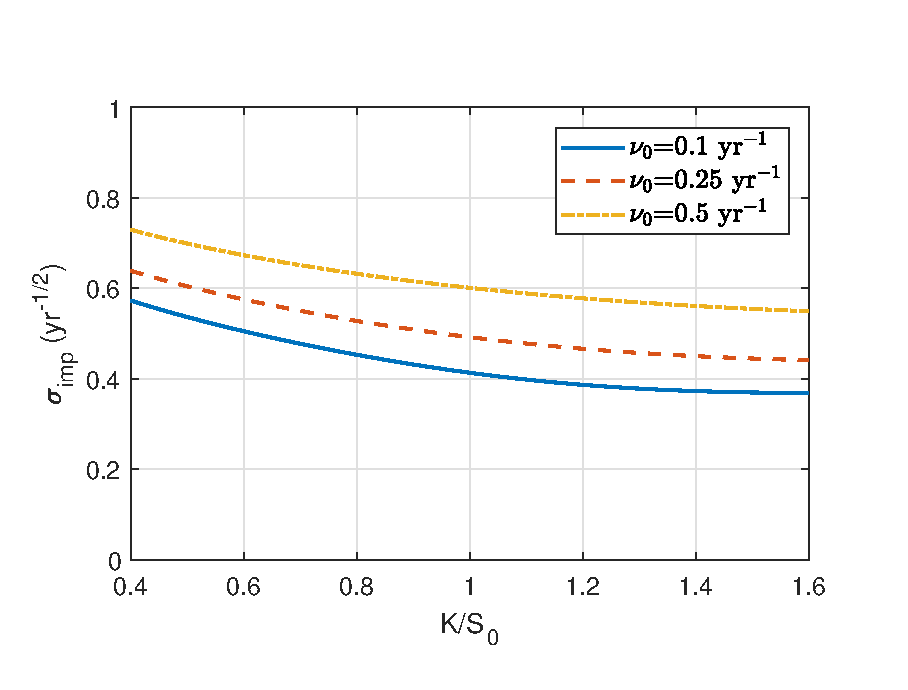
\includegraphics[width=0.49\linewidth,trim={0.25cm 0.45cm 1.1cm 1.4cm},clip]{Hnu0.eps}\label{Hn0}}
    \subfigure[Dependence on $\eta$]{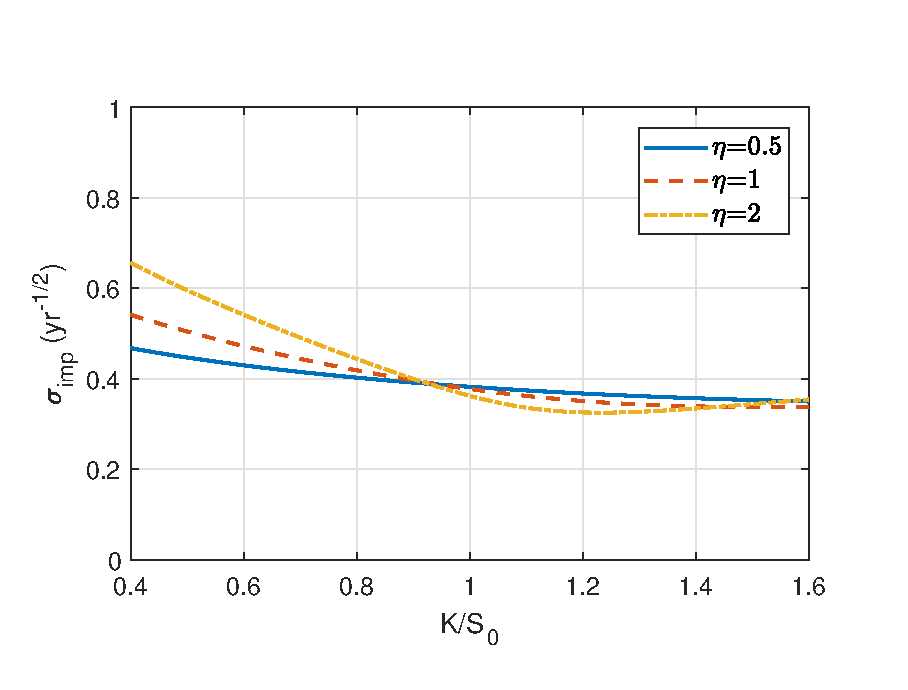
\includegraphics[width=0.49\linewidth,trim={0.25cm 0.45cm 1.1cm 1.4cm},clip]{Heta.eps}\label{He}}
        \subfigure[Dependence on $\rho$]{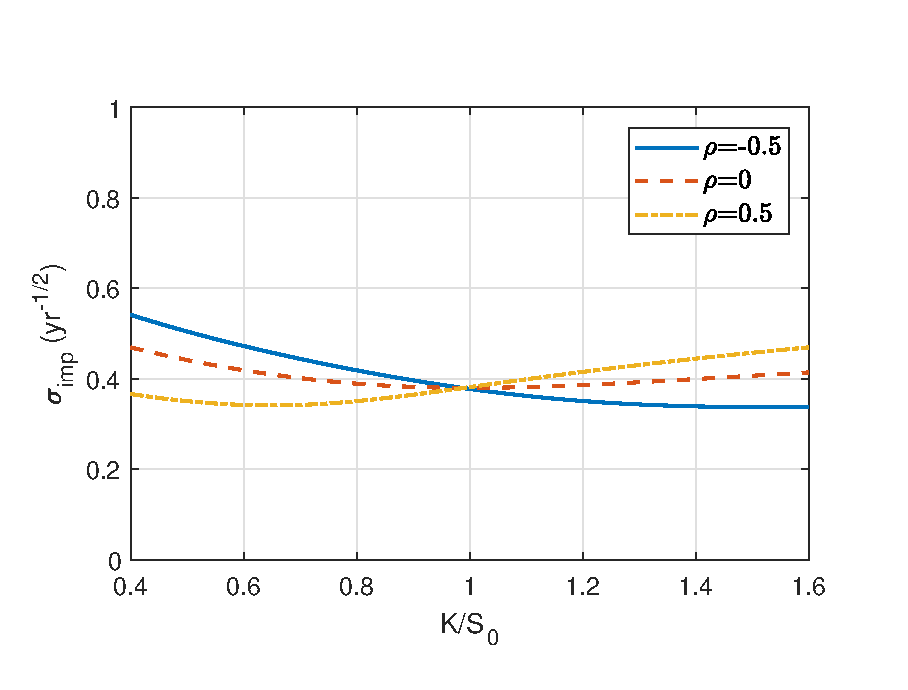
\includegraphics[width=0.49\linewidth,trim={0.25cm 0.45cm 1.1cm 1.4cm},clip]{Hrho.eps}\label{Hr}}
  \end{subfigmatrix}
  \caption[Dependence of the implied volatility curve on each of the Heston model parameters.]{Dependence of the implied volatility curve on each of the Heston model parameters. The default parameters used were $S_0=1\EUR$, $T=42$ days and $r=0$. Furthermore, on all plots, except when the dependence on a parameter is represented, the parameters used were $\kappa=10$, $\overline{\nu}=0.1$, $\nu_0=0.1$, $\eta=1$ and $\rho=-0.5$.}
  \label{fig:Hparam}
\end{figure}

The parameters $\kappa$, $\overline{\nu}$ and $\nu_0$ are inherently related and their influence can only be understood if all are considered at the same time. The parameter $\overline{\nu}$ is the mean value of the variance (\emph{not} the volatility! $\nu(t)=\sigma^2(t)$), $\nu_0$ denotes the initial variance, and $\kappa$ is the mean-reversion rate, which controls how fast the variance tends to its mean value.

If the parameter $\kappa$ is very large, we expect the variance process to converge very fast to its mean value, $\overline{\nu}$. This means that the variance process $\nu(t)$ is not able to change significantly, as it is stuck at $\overline{\nu}$, remaining roughly constant. For this reason, options priced with such parameters would have an almost constant \emph{volatility}, and their implied volatility curve would thus be a horizontal line equal to the square root of $\overline{\nu}$.

On the other hand, if $\kappa$ is small, the parameter $\overline{\nu}$ will barely have any influence at all on the implied volatility curve, and the variance process is able to change almost without restrain. This means that the parameter $\nu_0$ will have a large impact on the behavior of the variance process. A large $\nu_0$ enables the variance process to reach higher values (as does the equivalent process of volatility) so that the implied volatility of options priced with these parameters is higher. A small $\nu_0$ would have the opposite effect, decreasing the implied volatility.

If we now have a moderate value for $\kappa$, both parameters $\overline{\nu}$ and $\nu_0$ are expected to have some impact on the implied volatility curve.

By examining Figures \autoref{Hnb} and \autoref{Hn0}, with $\kappa=10$ (which is not too large nor too small), we see that the implied volatility curves increase/decrease as we increase/decrease each of the parameters, which is precisely what we expect.
If we now look at Figure \autoref{Hk}, we can confirm that a large value for $\kappa$ (orange dot-dashed line) will produce an almost constant implied volatility curve around the square root of $\overline{\nu}$ ($\sqrt{\overline{\nu}}=\sqrt{0.1}=...$).
\hl{change values of overline nu and nu0, change phrase below}
For small values of $\kappa$ (blue full line), the influence of the parameter $\nu_0$ becomes apparent (notice that the curve is pulled downwards since $\nu_0$ is lower than $\overline{\nu}$), and we no longer see the horizontal implied volatility curve from before, which is also expected.

The parameters $\eta$ and $\rho$ in the Heston model control the volatility of the variance process and the correlation of this process with the stock price process, respectively. They are very much related to the parameters $\nu$ and $\rho$ of the Static SABR process, respectively, and their impact on the implied volatility curve is the same. For this reason, they will not be discussed again here.


The Heston model was calibrated to the data provided using the closed form solutions described before. The calibrated parameters were then input into a Monte Carlo pricer and the simulated implied volatilities were obtained. These results are shown in \autoref{fig:H}.

\begin{figure}[H]
  \begin{subfigmatrix}{2}
    \subfigure[$T=21$ days]{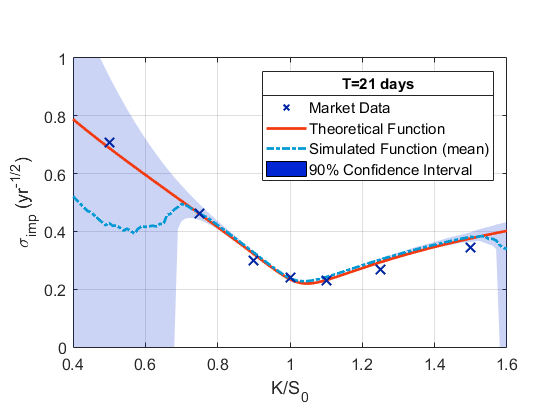
\includegraphics[width=0.49\linewidth,trim={0.25cm 0.45cm 1.1cm 1.4cm},clip]{H1.png}}
    \subfigure[$T=42$ days]{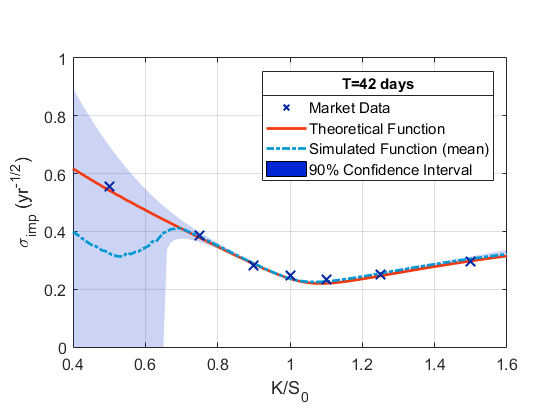
\includegraphics[width=0.49\linewidth,trim={0.25cm 0.45cm 1.1cm 1.4cm},clip]{H2.png}}
    \subfigure[$T=63$ days]{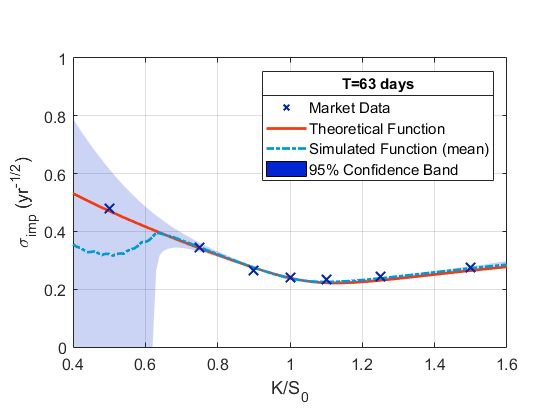
\includegraphics[width=0.49\linewidth,trim={0.25cm 0.45cm 1.1cm 1.4cm},clip]{H3.png}}
    \subfigure[$T=126$ days]{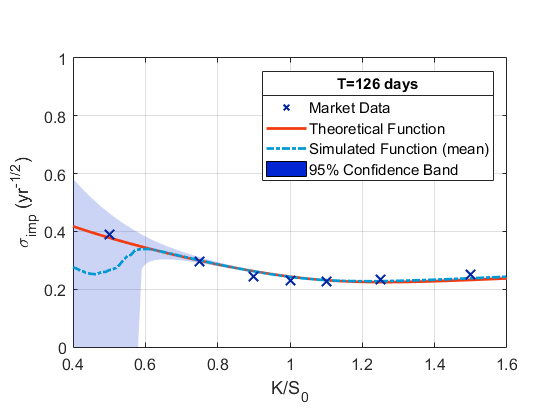
\includegraphics[width=0.49\linewidth,trim={0.25cm 0.45cm 1.1cm 1.4cm},clip]{H4.png}}
  \end{subfigmatrix}
  \caption[Implied volatility functions fitted simultaneously to the implied volatility data for different maturities under the Heston model, plotted with their respective Monte Carlo simulated functions along with their 95\% confidence intervals.]{Implied volatility functions (red lines) fitted simultaneously to the implied volatility data (crosses) for different maturities under the Heston model, plotted with their respective Monte Carlo simulated functions (light-blue dot-dashed lines) along with their 95\% confidence intervals (blue region).}
  \label{fig:H}
\end{figure}

The values of the calibrated parameters are shown in \autoref{tab:HR}.

\begin{table}[H]
    \centering
        \renewcommand{\arraystretch}{0.8}
\begin{tabular}{@{}lccccr@{}}
\toprule
$\kappa$ & $\overline{\nu}$ & $\nu_0$ & $\rho$ & $\eta$ & Cost \\ \midrule
53.4355 & 0.0653 & 0.1046 & -0.4086 & 6.2554 & 0.002529 \\
\bottomrule
\end{tabular}
  \caption[Fitted parameters for all maturities (fitted simultaneously) under the Heston model.]{Fitted parameters for all maturities (fitted simultaneously) under the Heston model.}
  \label{tab:HR}
\end{table}


We now study the results obtained. Examining the plots in \autoref{fig:H} we see that the theoretical curves fit the data surprisingly well throughout all the maturities.
This is especially surprising when we note that the adjustment is made for the entire data set, with all the different maturities.

Observing the simulated curves and their respective confidence intervals we again see that they fit the closed-form solutions extremely well in the region around $S_0$, indicating that the simulations agree with the predictions. The large confidence intervals described before for the high strikes and early maturities and for the low strikes can also be found here. Because their cause is the same, they will not be described again.

Considering now the cost function value for the fitted parameters (Cost$=0.002529$), shown in \autoref{tab:HR}, and comparing it to the sum of the costs of each of the independent fits in the Static SABR model ($\Sigma_{\mathrm{Costs}}=0.000415+0.000166+0.000102+0.000055=0.000738$), in \autoref{tab:SSR}, we note that the cost of the former is higher than that of the latter.
This is unsurprising, as the adjustments with the Static SABR were done independently of one another, and a better fit is therefore possible.

Comparing now the cost of the Heston model with that of the constant volatility assumption for dependent fits (Cost=$=0.1248$), shown in \autoref{tab:ConstVolPar2}, we see that our results improve by approximately $98\%$. The improvement is astonishing and completely justifies why the Heston model is so widely preferred over the constant volatility simplification.


Both the simulated and theoretical implied volatility curves shown in the plots of \autoref{fig:H} for different maturities can be thought of as slices of a implied volatility surfaces (one simulates, another theoretical). Similarly to what we did for the Dupire model, we again represent these surfaces and their respective contour plots in Figures \ref{fig:HS} and \ref{fig:HSSim}.


\begin{figure}[H]
  \begin{subfigmatrix}{2}
    \subfigure[$\sigma_{imp}$ surface]{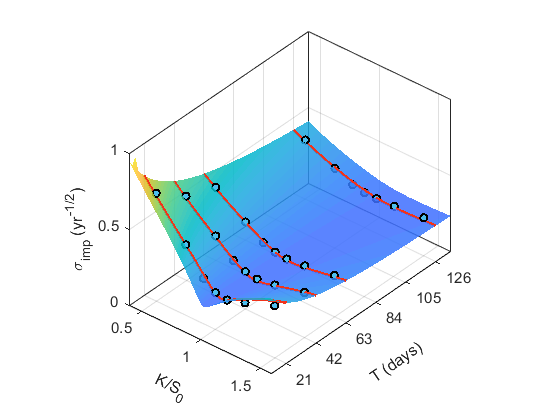
\includegraphics[width=0.49\linewidth,trim={1.7cm 0.45cm 2.35cm 0.85cm},clip]{HS.png}}
    \subfigure[$\sigma_{imp}$ contour plot]{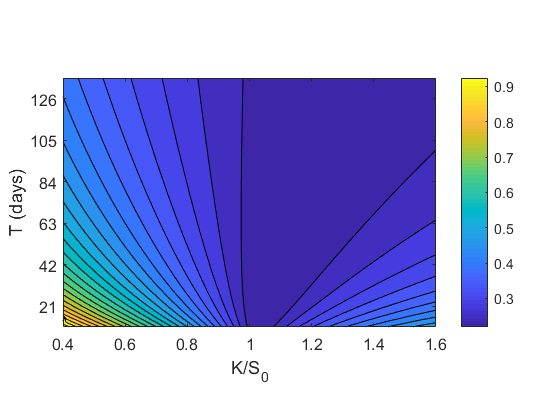
\includegraphics[width=0.49\linewidth,trim={0.2cm 0.5cm 1.25cm 1.55cm},clip]{HSC.png}}
  \end{subfigmatrix}
    \caption[Implied volatility surface and corresponding contour plot of the function fitted simmultaneously to the implied volatility data for different maturities under the Heston model, plotted against the original market data and the fitted functions shown in \autoref{fig:H}.]{Implied volatility surface (left) and corresponding contour plot (right) of the function fitted simmultaneously to the implied volatility data for different maturities under the Heston model, plotted against the original market data (blue circles) and the fitted functions shown in \autoref{fig:H} (red lines).}\label{fig:HS}
\end{figure}   


\begin{figure}[H]
  \begin{subfigmatrix}{2}
    \subfigure[$\sigma_{imp}$ surface]{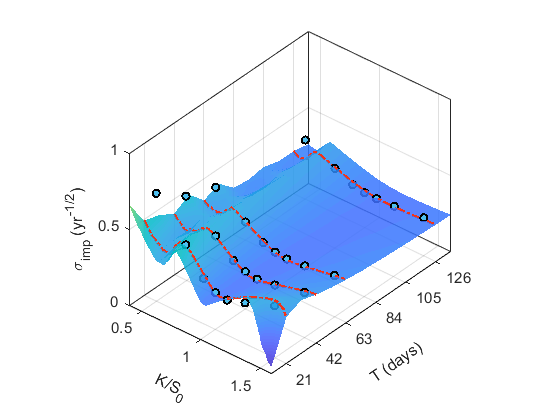
\includegraphics[width=0.49\linewidth,trim={1.7cm 0.45cm 2.35cm 0.85cm},clip]{HSSim.png}}
    \subfigure[$\sigma_{imp}$ contour plot]{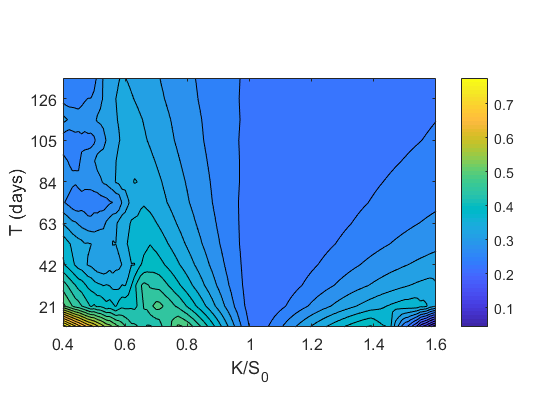
\includegraphics[width=0.49\linewidth,trim={0.2cm 0.5cm 1.25cm 1.55cm},clip]{HSCSim.png}}
  \end{subfigmatrix}
    \caption[Implied volatility surface and corresponding contour plot of the function simulated using the Monte Carlo procedure with the fitted parameters shown in \autoref{tab:HR}, under the Heston model, plotted against the original market data and the simulated functions shown in \autoref{fig:H}.]{Implied volatility surface (left) and corresponding contour plot (right) of the function simulated using the Monte Carlo procedure with the fitted parameters shown in \autoref{tab:HR}, under the Heston model, plotted against the original market data (blue circles) and the simulated functions shown in \autoref{fig:H} (red dot-dashed lines).}\label{fig:HSSim}
\end{figure} 


The surfaces and contour plots shown in Figures \ref{fig:HS} and \ref{fig:HSSim} should, ideally, replicate the surface and contour plot shown in \autoref{fig:DupImpV}, since these last correspond to the real (\emph{interpolated}) implied volatility surface. The simulated theoretical surface mimics the real function very well, which is expected, since the fits adjusted greatly to the data.
As for the simulated surface, we can see the expected noisy region for the low strikes. The region around $S_0$ fits rather well, however, as we can see from the comparison of the contour plots.


\begin{table}[H]
\centering
\renewcommand{\arraystretch}{0.8}
\begin{tabular}{@{}ccccSccS@{}}
\toprule
$T$(days) & $K$($\EUR$) & $\sigma_{i,\mathrm{mkt}}$($\SI{}{\year\tothe{-0.5}}$) &  $\sigma_{i,\mathrm{mdl}}$($\SI{}{\year\tothe{-0.5}}$) & \multicolumn{1}{c}{$\mathrm{Error}_{\sigma}(\%)$} & $C_{\mathrm{mkt}}$($\EUR$)&$C_{\mathrm{mdl}}$($\EUR$)& \multicolumn{1}{c}{$\mathrm{Error}_{C}(\%)$}\\ \midrule
\multirow{7}{*}{21} & 0.50 & 0.7082 & 0.6886 & 2.8 & 0.50001 & 0.50001 & 0.001 \\
 & 0.75 & 0.4632 & 0.4604 & 0.6 & 0.25065 & 0.25062 & 0.01 \\
 & 0.90 & 0.2989 & 0.3216 & 7.6 & 0.10439 & 0.10563 & 1.2 \\
 & 1.00 & 0.2425 & 0.2346 & 3.2 & 0.02792 & 0.02702 & 3.2 \\
 & 1.10 & 0.2314 & 0.2316 & 0.1 & 2.42$\times10^{-3}$ & 2.43$\times10^{-3}$ & 0.3 \\
 & 1.25 & 0.2699 & 0.2935 & 8.7 & 5.34$\times10^{-5}$ & 12.43$\times10^{-5}$ & 132.5 \\
 & 1.50 & 0.3433 & 0.3759 & 9.5 & 5.75$\times10^{-7}$ & 29.58$\times10^{-7}$ & 414.7 \\\midrule
\multirow{7}{*}{42} & 0.50 & 0.5556 & 0.5422 & 2.4 & 0.50005 & 0.50004 & 0.003 \\
 & 0.75 & 0.3876 & 0.3781 & 2.5 & 0.25186 & 0.25162 & 0.1 \\
 & 0.90 & 0.2824 & 0.2873 & 1.7 & 0.11069 & 0.11120 & 0.5 \\
 & 1.00 & 0.2461 & 0.2366 & 3.9 & 0.04006 & 0.03852 & 3.9 \\
 & 1.10 & 0.2354 & 0.2205 & 6.3 & 8.52$\times10^{-3}$ & 7.02$\times10^{-3}$ & 17.6 \\
 & 1.25 & 0.2525 & 0.2463 & 2.4 & 6.21$\times10^{-4}$ & 5.20$\times10^{-4}$ & 16.2 \\
 & 1.50 & 0.2968 & 0.2979 & 0.4 & 1.58$\times10^{-5}$ & 1.66$\times10^{-5}$ & 4.9 \\\midrule
\multirow{7}{*}{63} & 0.50 & 0.4789 & 0.4709 & 1.7 & 0.50009 & 0.50008 & 0.003 \\
 & 0.75 & 0.3452 & 0.3420 & 0.9 & 0.25296 & 0.25282 & 0.1 \\
 & 0.90 & 0.2658 & 0.2748 & 3.4 & 0.11533 & 0.11659 & 1.1 \\
 & 1.00 & 0.2401 & 0.2392 & 0.4 & 0.04787 & 0.04768 & 0.4 \\
 & 1.10 & 0.2330 & 0.2224 & 4.6 & 0.01421 & 0.01265 & 11.0 \\
 & 1.25 & 0.2438 & 0.2310 & 5.2 & 1.80$\times10^{-3}$ & 1.31$\times10^{-3}$ & 27.1 \\
 & 1.50 & 0.2749 & 0.2649 & 3.7 & 7.66$\times10^{-5}$ & 4.97$\times10^{-5}$ & 35.1 \\\midrule
\multirow{7}{*}{126} & 0.50 & 0.3878 & 0.3784 & 2.4 & 0.50035 & 0.50028 & 0.01 \\
 & 0.75 & 0.2954 & 0.2993 & 1.3 & 0.25694 & 0.25732 & 0.1 \\
 & 0.90 & 0.2444 & 0.2626 & 7.5 & 0.12716 & 0.13124 & 3.2 \\
 & 1.00 & 0.2295 & 0.2439 & 6.3 & 0.06467 & 0.06870 & 6.2 \\
 & 1.10 & 0.2269 & 0.2314 & 2.0 & 0.02862 & 0.02973 & 3.9 \\
 & 1.25 & 0.2340 & 0.2248 & 3.9 & 7.57$\times10^{-3}$ & 6.45$\times10^{-3}$ & 14.8 \\
 & 1.50 & 0.2521 & 0.2324 & 7.8 & 8.58$\times10^{-4}$ & 4.45$\times10^{-4}$ & 48.2 \\ 
 \bottomrule
\end{tabular}
  \caption[Comparison between fitted results and original data under the Heston model.]{Comparison between fitted results and original data under the Heston model.}
  \label{tab:H}
\end{table}











\newpage

\section{Dynamic SABR Model}

The Dynamic SABR Model was defined as
\begin{equation}
dS(t)=rS(t)dt+e^{-r(T-t)(1-\beta)}\sigma(t) (S(t))^\beta dW_1(t),
\end{equation}
\begin{equation}
d\sigma(t)=\nu(t)\sigma(t) dW_2(t),
\end{equation}
\noindent with the volatility of the volatility process, $\nu(t)$, and the correlation between $W_1(t)$ and $W_2(t)$, $\rho(t)$, being two functions of time.

To model these functions we chose
\begin{equation}
\rho(t)=\rho_0e^{-at},
\end{equation}
\begin{equation}
\nu(t)=\nu_0e^{-bt},
\end{equation}
\noindent with $\rho_0\in[-1,1]$, $\nu_0>0$, $a>0$ and $b>0$.

With these assumptions, the closed form solution of the implied volatility of options priced under this model was given in eq.\eqref{dynsabr}.

The parameters used in the Dynamic SABR model are similar to those used in the Static SABR model and an easy connection can be made between them. Their influence on the implied volatility curve will therefore be the same and, for this reason, we will not consider it again here.

We fitted the Dynamic SABR model to the implied volatility data for all maturities. The fitted theoretical curves (obtained with the closed-form solution) and their simulated counterparts are shown in \autoref{fig:DS}.




\begin{figure}[H]
  \begin{subfigmatrix}{2}
    \subfigure[$T=21$ days]{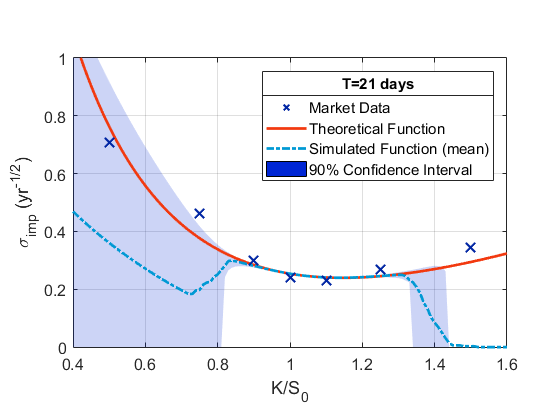
\includegraphics[width=0.49\linewidth,trim={0.25cm 0.45cm 1.1cm 1.4cm},clip]{DS1.png}}
    \subfigure[$T=42$ days]{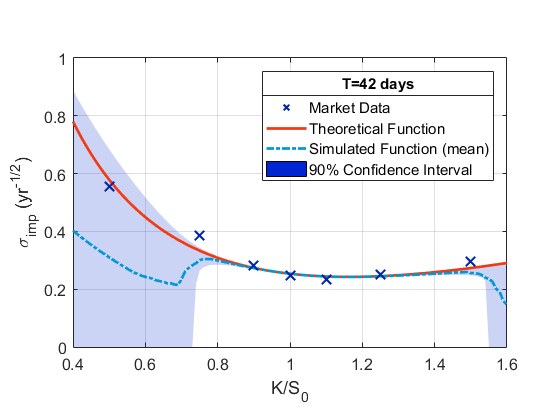
\includegraphics[width=0.49\linewidth,trim={0.25cm 0.45cm 1.1cm 1.4cm},clip]{DS2.png}}
    \subfigure[$T=63$ days]{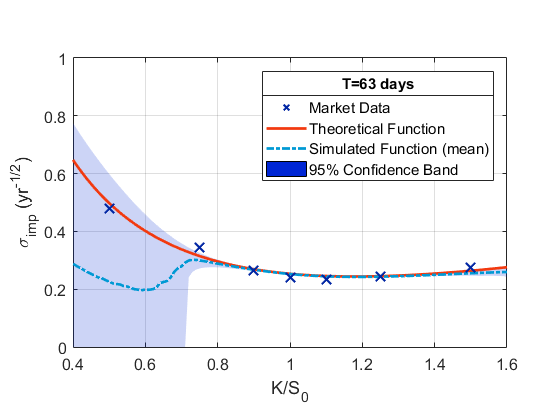
\includegraphics[width=0.49\linewidth,trim={0.25cm 0.45cm 1.1cm 1.4cm},clip]{DS3.png}}
    \subfigure[$T=126$ days]{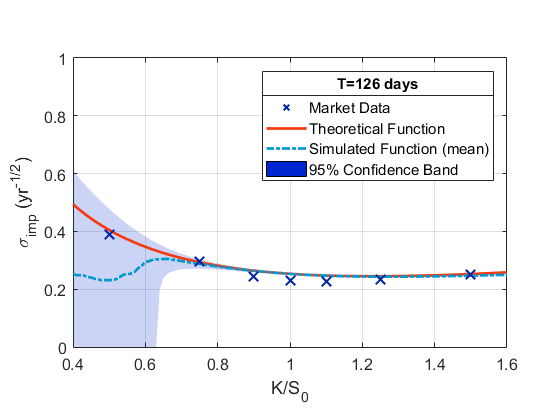
\includegraphics[width=0.49\linewidth,trim={0.25cm 0.45cm 1.1cm 1.4cm},clip]{DS4.png}}
  \end{subfigmatrix}
  \caption[Implied volatility functions fitted simultaneously to the implied volatility data for different maturities under the dynamic SABR model, plotted with their respective Monte Carlo simulated functions along with their 95\% confidence intervals.]{Implied volatility functions (red lines) fitted simultaneously to the implied volatility data (crosses) for different maturities under the dynamic SABR model, plotted with their respective Monte Carlo simulated functions (light-blue dot-dashed lines) along with their 95\% confidence intervals (blue region).}
  \label{fig:DS}
\end{figure}

The calibrated parameters obtained from the fit are shown in \autoref{tab:DSR}.

\begin{table}[H]
    \centering
        \renewcommand{\arraystretch}{0.8}
\begin{tabular}{@{}lcccccr@{}}
\toprule
$\alpha$ & $\beta$ & $\rho_0$ & $a$ & $\nu_0$ & $b$ & Cost \\ \midrule
0.2540 & 0.6348 & -0.4166 & 0 & 1.8673 & 41.6943 & 0.0108 \\
\bottomrule
\end{tabular}
  \caption[Fitted parameters for all maturities (fitted simultaneously) under the dynamic SABR model.]{Fitted parameters for all maturities (fitted simultaneously) under the dynamic SABR model.}
  \label{tab:DSR}
\end{table}


We now consider the adjustments above. Observing the theoretical curves in \autoref{fig:DS} we can see that they fit the market data relatively well, especially for the later maturities. For the maturity of 21 days, the theoretical curve doesn't seem to follow the market values accurately, however. Comparing these results with those obtained with the Heston model, we see that Dynamic SABR actually performs worse.

Considering now the simulated curves, we again see that they accurately follow the theoretical curve for the regions around $S_0$, behaving very badly for the low strike regions and for high strikes with low maturities. This has been observed before in all models and is therefore expected.

If we now compare the cost function of the Dynamic SABR model (Cost$=0.0108$), shown in \autoref{tab:DSR}, with the sum of the costs of the independent fits for the Static SABR ($\Sigma_{\mathrm{Costs}}=0.000415+0.000166+0.000102+0.000055=0.000738$), in \autoref{tab:SSR}, the former is much greater than that of the latter.
This is unsurprising, since the Static SABR fits only a small amount of data for a single maturity and Dynamic SABR attempts to model a whole surface.

Comparing the cost resulting from the Heston model (Cost$=0.002529$) with that from Dynamic SABR, we see that even though both models fit the same data on a range of different maturities, Heston outperforms the Dynamic SABR quite significantly. This was expected from the comparison of the theoretical functions in Figures \ref{fig:H} and \ref{fig:DS}.

Finally comparing cost of the Dynamic SABR model with the constant volatility assumption for dependent fits (Cost=$=0.1248$), shown in \autoref{tab:ConstVolPar2}, the results improve by approximately $91\%$, compared to the $98\%$ improvement seen with the Heston model. Despite performing worse than Heston, the improvement against the constant volatility model is still striking.

As we did for the Heston model, we now present the theoretical and simulated implied volatility surfaces of which the plots in \autoref{fig:DS} are slices. 
These surfaces and their respective contour plots are shown in Figures \ref{fig:DSS} and \ref{fig:DSSSim}.



\begin{figure}[H]
  \begin{subfigmatrix}{2}
    \subfigure[$\sigma_{imp}$ surface]{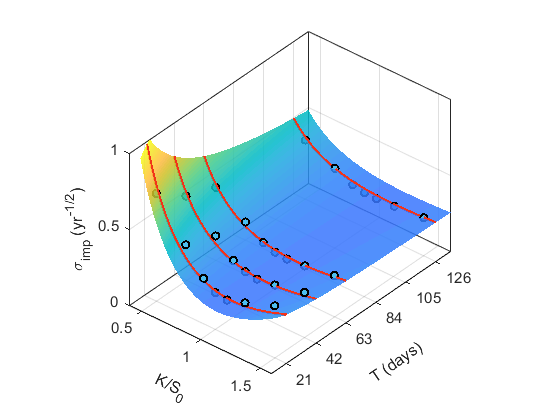
\includegraphics[width=0.49\linewidth,trim={1.7cm 0.45cm 2.35cm 0.85cm},clip]{DSS.png}}
    \subfigure[$\sigma_{imp}$ contour plot]{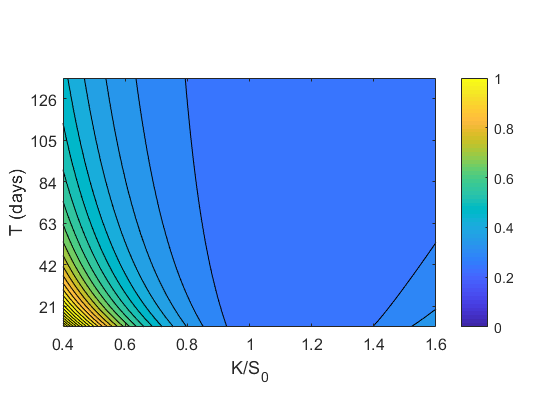
\includegraphics[width=0.49\linewidth,trim={0.2cm 0.5cm 1.25cm 1.55cm},clip]{DSSC.png}}
  \end{subfigmatrix}
    \caption[Implied volatility surface and corresponding contour plot of the function fitted simmultaneously to the implied volatility data for different maturities under the dynamic SABR model, plotted against the original market data and the fitted functions shown in \autoref{fig:DS}.]{Implied volatility surface (left) and corresponding contour plot (right) of the function fitted simmultaneously to the implied volatility data for different maturities under the dynamic SABR model, plotted against the original market data (blue circles) and the fitted functions shown in \autoref{fig:DS} (red lines).}\label{fig:DSS}
\end{figure}   


\begin{figure}[H]
  \begin{subfigmatrix}{2}
    \subfigure[$\sigma_{imp}$ surface]{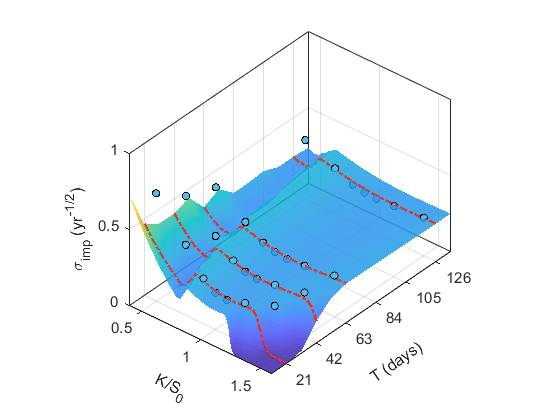
\includegraphics[width=0.49\linewidth,trim={1.7cm 0.45cm 2.35cm 0.85cm},clip]{DSSSim.png}}
    \subfigure[$\sigma_{imp}$ contour plot]{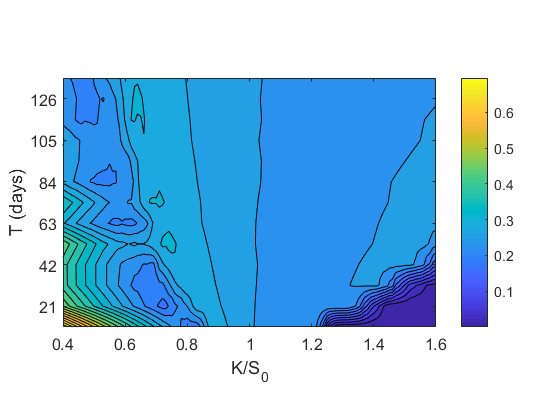
\includegraphics[width=0.49\linewidth,trim={0.2cm 0.5cm 1.25cm 1.55cm},clip]{DSSCSim.png}}
  \end{subfigmatrix}
    \caption[Implied volatility surface and corresponding contour plot of the function simulated using the Monte Carlo procedure with the fitted parameters shown in \autoref{tab:DSR}, under the dynamic SABR model, plotted against the original market data and the simulated functions shown in \autoref{fig:DS}.]{Implied volatility surface (left) and corresponding contour plot (right) of the function simulated using the Monte Carlo procedure with the fitted parameters shown in \autoref{tab:DSR}, under the dynamic SABR model, plotted against the original market data (blue circles) and the simulated functions shown in \autoref{fig:DS} (red dot-dashed lines).}\label{fig:DSSSim}
\end{figure} 


As stated before, ideally the plots in these two Figures would perfectly mimic the surface shown in \autoref{fig:DupImpV}. This obviously doesn't occur. The theoretical surface plot in \autoref{fig:DSS} seems to be flatter than the actual surface in the regions around $S_0$ (notice the wider contours in this region) whereas it increases quite abruptly for low strikes.
As for the simulated surface in \autoref{fig:DSSSim}, the surface is heavily modified by noise, which is expected from the adjustments shown before.

\begin{table}[H]
\centering
\renewcommand{\arraystretch}{0.8}
\begin{tabular}{@{}ccccSccS@{}}
\toprule
$T$(days) & $K$($\EUR$) & $\sigma_{i,\mathrm{mkt}}$($\SI{}{\year\tothe{-0.5}}$) &  $\sigma_{i,\mathrm{mdl}}$($\SI{}{\year\tothe{-0.5}}$) & \multicolumn{1}{c}{$\mathrm{Error}_{\sigma}(\%)$} & $C_{\mathrm{mkt}}$($\EUR$)&$C_{\mathrm{mdl}}$($\EUR$)& \multicolumn{1}{c}{$\mathrm{Error}_{C}(\%)$}\\ \midrule
\multirow{7}{*}{21} & 0.50 & 0.7082 & 0.7625 & 7.7 & 0.50001 & 0.50003 & 0.004 \\
 & 0.75 & 0.4632 & 0.3765 & 18.7 & 0.25065 & 0.25012 & 0.2 \\
 & 0.90 & 0.2989 & 0.2843 & 4.9 & 0.10439 & 0.10367 & 0.7 \\
 & 1.00 & 0.2425 & 0.2540 & 4.7 & 0.02792 & 0.02924 & 4.7 \\
 & 1.10 & 0.2314 & 0.2410 & 4.2 & 2.42$\times10^{-3}$ & 2.86$\times10^{-3}$ & 18.0 \\
 & 1.25 & 0.2699 & 0.2454 & 9.1 & 5.34$\times10^{-5}$ & 1.76$\times10^{-5}$ & 67.1 \\
 & 1.50 & 0.3433 & 0.2944 & 14.2 & 57.48$\times10^{-8}$ & 1.86$\times10^{-8}$ & 96.8 \\\midrule
\multirow{7}{*}{42} & 0.50 & 0.5556 & 0.5788 & 4.2 & 0.50005 & 0.50008 & 0.01 \\
 & 0.75 & 0.3876 & 0.3337 & 13.9 & 0.25186 & 0.25074 & 0.4 \\
 & 0.90 & 0.2824 & 0.2740 & 3.0 & 0.11069 & 0.10985 & 0.8 \\
 & 1.00 & 0.2461 & 0.2538 & 3.1 & 0.04006 & 0.04131 & 3.1 \\
 & 1.10 & 0.2354 & 0.2445 & 3.9 & 8.52$\times10^{-3}$ & 9.49$\times10^{-3}$ & 11.3 \\
 & 1.25 & 0.2525 & 0.2455 & 2.8 & 6.21$\times10^{-4}$ & 5.07$\times10^{-4}$ & 18.3 \\
 & 1.50 & 0.2968 & 0.2736 & 7.8 & 15.83$\times10^{-6}$ & 4.72$\times10^{-6}$ & 70.2 \\\midrule
\multirow{7}{*}{63} & 0.50 & 0.4789 & 0.4980 & 4.0 & 0.50009 & 0.50014 & 0.01 \\
 & 0.75 & 0.3452 & 0.3150 & 8.8 & 0.25296 & 0.25182 & 0.5 \\
 & 0.90 & 0.2658 & 0.2695 & 1.4 & 0.11533 & 0.11585 & 0.4 \\
 & 1.00 & 0.2401 & 0.2537 & 5.7 & 0.04787 & 0.05057 & 5.6 \\
 & 1.10 & 0.2330 & 0.2460 & 5.6 & 0.01421 & 0.01619 & 13.9 \\
 & 1.25 & 0.2438 & 0.2455 & 0.7 & 1.80$\times10^{-3}$ & 1.87$\times10^{-3}$ & 3.8 \\
 & 1.50 & 0.2749 & 0.2642 & 3.9 & 7.66$\times10^{-5}$ & 4.81$\times10^{-5}$ & 37.2 \\\midrule
\multirow{7}{*}{126} & 0.50 & 0.3878 & 0.4050 & 4.4 & 0.50035 & 0.50051 & 0.03 \\
 & 0.75 & 0.2954 & 0.2935 & 0.6 & 0.25694 & 0.25677 & 0.1 \\
 & 0.90 & 0.2444 & 0.2645 & 8.2 & 0.12716 & 0.13168 & 3.6 \\
 & 1.00 & 0.2295 & 0.2537 & 10.5 & 0.06467 & 0.07147 & 10.5 \\
 & 1.10 & 0.2269 & 0.2477 & 9.1 & 0.02862 & 0.03382 & 18.2 \\
 & 1.25 & 0.2340 & 0.2452 & 4.8 & 7.57$\times10^{-3}$ & 9.05$\times10^{-3}$ & 19.6 \\
 & 1.50 & 0.2521 & 0.2528 & 0.3 & 8.58$\times10^{-4}$ & 8.77$\times10^{-4}$ & 2.3 \\
 \bottomrule
\end{tabular}
  \caption[Comparison between fitted results and original data under the dynamic SABR model.]{Comparison between fitted results and original data under the dynamic SABR model.}
  \label{tab:DS}
\end{table}





\section{Mishaps Found in Implementation}
During the implementation of all the models, some problems were found. They were all solved and the models were able to perform as expected, as we saw in the previous section. For future reference, and to prevent others from repeating the same problems, we now summarize not only the problems observed but also their causes and how we were able to solve them.

\subsection{Dupire Model}
While implementing the Dupire model we noticed that the local volatility surface produced by the model was heavily dependent on the chosen interpolation method. Moreover, we found that it was particularly sensitive to the intervals $\Delta K$ and $\Delta T$ chosen in the interpolation. If chosen to be too large, the gradients wouldn't be able to capture the surface curvature and the local volatility surface would look unrealistic. If chosen to be too small, because we used Delaunay's triangulation method as interpolation, which creates triangular planes between three points, the second derivative would be zero if $K$, $K+\Delta K$ and $K-\Delta K$ were all evaluated inside the same triangle, which is bound to be true for the majority of points if $\Delta K$ is small enough. This would output a wrong second derivative.
Thus, the intervals $\Delta K$ and $\Delta T$ have to be chosen very carefully.

As an example, in \autoref{fig:DupBad} we present how different choices for these intervals affects the local volatility surface.

\begin{figure}[H]
  \begin{subfigmatrix}{2}
    \subfigure[bla bla bla bla]{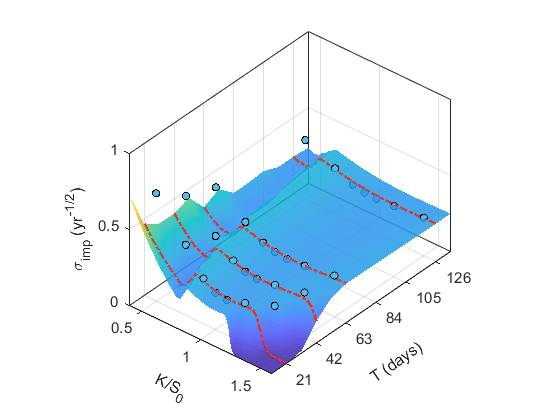
\includegraphics[width=0.49\linewidth,trim={1.7cm 0.45cm 2.35cm 0.85cm},clip]{DSSSim.png}}
    \subfigure[bla bla bla bla]{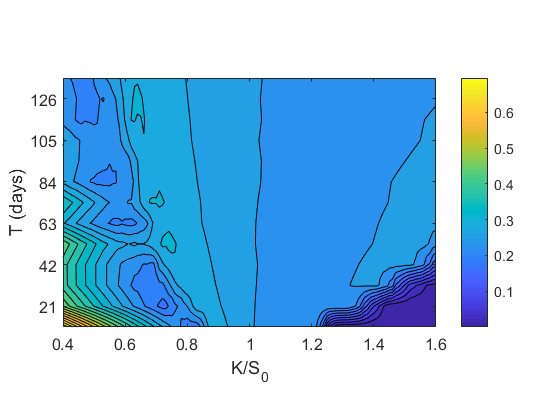
\includegraphics[width=0.49\linewidth,trim={0.2cm 0.5cm 1.25cm 1.55cm},clip]{DSSCSim.png}}
  \end{subfigmatrix}
    \caption[Bla bla bla bla]{Bla bla bla bla}\label{fig:DupBad}
\end{figure} 

There exist two possible alternatives to solve this problem.
On the one hand, we could significantly increase the number of data points. This would ensure that the triangle size from Delaunay's triangulation is small enough for the numerical second derivative to produce realistic results. The problem is that more data isn't always available, and this alternative may not be possible.
The other possible path, which was the one chosen in this work, is to test several values for the intervals and observe which of them produces the most realistic gradients and the most realistic local volatility surface. This alternative has the caveat that the choice for the intervals is very subjective.

\subsection{Heston Model}
In the Heston model, we need to evaluate some integrals to find the closed-form solutions of call prices.
These integrals are evaluated between $0$ and $\infty$, and because they are not analytically solvable, they have to be calculated numerically.
We thus obviously need to define some numerical limits for the integrals, since numerical integration until $\infty$ is impossible. Cui \textit{et al.}\citep{Cui} showed that these integrals only have to be evaluated until a $u\approx100$, because the integrands decrease fast enough that they become negligible after this point. During our implementation, this threshold proved to be insufficient when we evaluated the integrals for the earliest maturity with strikes far below and far above $S_0$. For such regions, some erratic oscillating behavior was found, which we represent in \autoref{fig:Hbad}.

\begin{figure}[H]
  \begin{subfigmatrix}{2}
    \subfigure[bla bla bla bla]{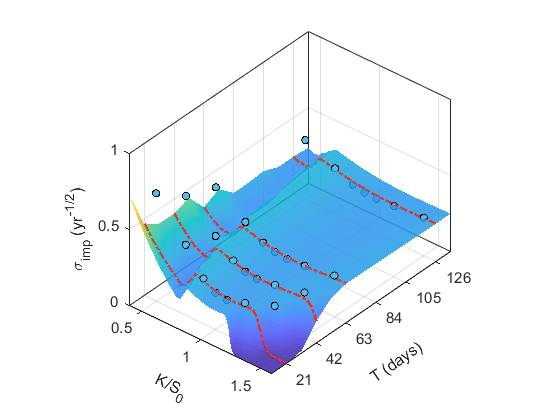
\includegraphics[width=0.49\linewidth,trim={1.7cm 0.45cm 2.35cm 0.85cm},clip]{DSSSim.png}}
    \subfigure[bla bla bla bla]{\includegraphics[width=0.49\linewidth,trim={0.2cm 0.5cm 1.25cm 1.55cm},clip]{DSSCSim.png}}
  \end{subfigmatrix}
    \caption[Bla bla bla bla]{Bla bla bla bla}\label{fig:Hbad}
\end{figure} 

This problem was solved simply by increasing the integration limits until $xxxx$ \hl{put integration limit here}.



\subsection{SABR Model}
One problem related to the SABR models is the fact that stock prices might become negative, which is unrealistic. This event is very rare and was usually only found in one of the simulated paths out of 100000.
The reason why this problem only occurred for the SABR models and not for Heston is due to the fact that the volatility process in the former is not mean reverting.
This detail enables the volatility process to evolve without restrain. If the volatility process becomes extremely large, the jumps in the stock price process become also very large. In the limit, it is perfectly possible that one of these jumps decreases the stock price process past zero. For the Heston model this problem is not observed because the volatility process (we used the variance process, but they are equivalent) is mean-reverting, so that the volatility doesn't evolve unrestrained.

This negative price shortcoming is more problematic in the SABR model because in the stock price process one of the terms is a stock price with an exponent $\beta$. If $\beta\neq0$ and $\beta\neq1$ and $S(t)<0$, this process will become complex, and the whole pricing procedure fails.

To solve this problem we simply cut the negative stock price paths to zero, preventing them from becoming negative.



\subsection{Other Problems}
During the implementation we also found that, in the Monte Carlo siimulations, updating the volatility process before the stock price produced results that didn't match the theoretical predictions in both the Heston and SABR models.

In other words, if we used
\begin{equation}
S(t+\Delta t)=\sigma(t+\Delta t).\left(\ldots\right)+\ldots,
\end{equation}
instead of the correct
\begin{equation}
S(t+\Delta t)=\sigma(t).\left(\ldots\right)+\ldots,
\end{equation}
\noindent the results obtained become wrong.
This is expected because the whole correlation mechanism, relating the two stochastic processes through the variable $\rho$, falls apart when we use the first formula.

\section{Barrier Options}

The Monte Carlo algorithms developed to price the European options in the previous sections under each of the models can be easily adapted to price Barrier options.
We are only required to check at each time step if the stock price process crossed the barrier level or not and, at the maturity, only keep the processes that did. This discretization poses a problem when pricing Barrier options, because these contracts assume a continuous time frame. This has been discussed in \autoref{subsection:Simulating stock prices}. Furthermore, as we discussed in \autoref{subsection:Pricing options from simulations}, the problem we observed before with the low number of simulated paths contributing to the price of an option with a very high strike and an early maturity is further aggravated with this Exotic option contract.

Despite these expected shortcomings, we priced several Barrier options with different barrier levels and under the all the different models described before. In these simulations we assumed a single maturity of 21 days and the calibrated parameters for each of the models, shown earlier in this Chapter. The results of these simulations are shown in \autoref{fig:Barrier}.

\begin{figure}[H]
  \begin{subfigmatrix}{2}
    \subfigure[bla bla bla bla]{\includegraphics[width=0.49\linewidth,trim={1.7cm 0.45cm 2.35cm 0.85cm},clip]{DSSSim.png}}
    \subfigure[bla bla bla bla]{\includegraphics[width=0.49\linewidth,trim={0.2cm 0.5cm 1.25cm 1.55cm},clip]{DSSCSim.png}}
  \end{subfigmatrix}
    \caption[Bla bla bla bla]{Bla bla bla bla}\label{fig:Barrier}
\end{figure} 

\newpage

\hlc[green]{in the tables show only one maturity and show the simulation implied vols, deleting the option prices (or showing in a different table)}

\hlc[green]{create a cost function for the simulated volatility functions besides the already existing cost for the theoretical values, in order to compare dupire's model}

\hlc[green]{plot the decaying functions of rho and nu on the dynamic sabr model}

\hlc[green]{check with Claude if BNPP data assumes a 0 interest rate or not}

\hlc[green]{ask prof Dilao why we use the forward gradient wrt time in the dupire interpolation gradient}

\hlc[red]{why is the coupled constant implied volatility the average of the independent fits of the constant implied vols?}

\hlc[red]{dynamic sabr exponential functions for rho should match the data for the individual fits}

\hlc[red]{mention the implied vol sensitivity to option price but changing maturity.}

\hlc[red]{how is extrapolation done in dupires model}

\hlc[red]{explain why static sabr only works for one maturity}


\hl{check notation:}

$\sigma_{i,\mathrm{mkt}}$ vs $\sigma_{imp,\mathrm{mkt}}$;

\hl{put units in fitted parameters}


\hl{in the plots of the chapters background and implementation, use dashed and dot-dashed lines}

\hl{save files as .png}

\hl{change labels from "simulated function" to something else}

\hl{check number of decimal places in the parameters tables (in particular for the cost function value)}

\hl{in multiple volatilities plot, check the label}

\hl{explain how the  lower bound volatility sensitivity plot was obtained}

\hl{explain what C means in the lower bound volatility sensitivity plot}

\hl{redo fokker-planck proof}

\hl{redo heston proof}

\hl{in heston proof, show ito's lemma for two dimensions}

\hl{change the 3d surface captions of the blue circles to something else}

\hl{in dupire's results table, the implied volatilities should have subscript "sim" instead of "mdl"}

\hl{replot the parameter influence in Heston}

\hl{put 95 percent confidence intervals}

\hl{put proof of option price lower bound}

\hl{in plot of implied vol vs. option price, put C mkt in axis label}

\hl{put year in all bibliographic references}